\documentclass[12pt, a4 paper]{article}
% Set target color model to RGB
\usepackage[inner=2.5cm,outer=2.5cm,top=3cm,bottom=3cm]{geometry}
\usepackage{setspace}
\usepackage{verbatim}
\usepackage{subcaption}
\usepackage{amsgen,amsmath,amstext,amsbsy,amsopn,tikz,amssymb}
\usepackage{bbm}
\usepackage{fancyhdr}
\usepackage[colorlinks=true, urlcolor=blue,  linkcolor=blue, citecolor=blue]{hyperref}
\usepackage{subcaption}
\usepackage{sectsty}
\hypersetup{%
pdfauthor={Abijith J Kamath},%
pdftitle={Homework},%
pdfkeywords={Tikz,latex,bootstrap,uncertaintes},%
pdfcreator={PDFLaTeX},%
pdfproducer={PDFLaTeX},%
}

\newcommand{\ra}[1]{\renewcommand{\arraystretch}{#1}}

\newtheorem{thm}{Theorem}[section]
\newtheorem{prop}[thm]{Proposition}
\newtheorem{lem}[thm]{Lemma}
\newtheorem{cor}[thm]{Corollary}
\newtheorem{defn}[thm]{Definition}
\newtheorem{rem}[thm]{Remark}
\numberwithin{equation}{section}

\newcommand{\homework}[6]{
   \pagestyle{myheadings}
   \thispagestyle{plain}
   \newpage
   \setcounter{page}{1}
   \noindent
   \begin{center}
   \framebox{
      \vbox{\vspace{2mm}
    \hbox to 6.28in { {\bf E1 213:~Pattern Recognition and Neural Networks\hfill {\small Spring 2021}} }
       \vspace{6mm}
       \hbox to 6.28in { {\bfseries \Large \hfill #1  \hfill} }
       \vspace{6mm}
       \hbox to 6.28in { {\it Author: {\rm Abijith J. Kamath}} \hfill {\small {\it Email:} abijithj@iisc.ac.in}}
      \vspace{2mm}}
   }
   \end{center}
   \markboth{E1 213 -- #1}{E1 213 -- #1}
   \vspace*{4mm}
}

\newcommand{\problem}[1]{~\\\fbox{\textbf{#1}}\newline\newline}
\newcommand{\subproblem}[1]{~\newline\textbf{(#1)}}

\newcommand{\solution}{~\newline\textbf{\textit{(Solution)}} }

\linespread{1.3}

\setlength{\intextsep}{20pt} % Vertical space above & below [h] floats
\setlength{\textfloatsep}{20pt} % Vertical space below (above) [t] ([b]) floats
\setlength{\abovecaptionskip}{10pt}
\setlength{\belowcaptionskip}{10pt}

\newcommand{\by}{\mathbf{y}}
\newcommand{\bx}{\mathbf{x}}
\newcommand{\bX}{\mathbf{X}}
\newcommand{\bW}{\mathbf{W}}
\newcommand{\bA}{\mathbf{A}}
\newcommand{\bF}{\mathbf{F}}
\newcommand{\rr}{\mathbb{R}}
\newcommand{\cc}{\mathbb{C}}
\newcommand{\Ex}{\mathbb{E}}
\newcommand{\TT}{\mathsf{T}}
\newcommand{\HH}{\mathsf{H}}

\newcommand{\bmu}{\boldsymbol{\mu}}
\newcommand{\btheta}{\boldsymbol{\theta}}
\newcommand{\bSigma}{\boldsymbol{\Sigma}}

\chapterfont{\fontfamily{lmss}\selectfont}
\sectionfont{\fontfamily{lmss}\selectfont}
\subsectionfont{\fontfamily{lmss}\selectfont}

\begin{document}
\homework{Assignment 1: Implementing Bayes' Classifier}{}




\section*{Introduction}
\label{sec:intro}

Let patterns be in $\rr^d$ and consider the $2$-class classification problem -- given a pattern $\bx$, classify the pattern into a class with label $y$. In Bayesian classification theory, the training data $\{\bx^{(i)}, y^{(i)}\}_{i=1}^n$ is viewed to be i.i.d samples of the random vector $(\bX, Y)$. The training samples are used to model the joint distribution of the random vector $(\bX, Y)$. \\

Let $\Pr(C_i) = p_i$ be the priors associated with the $i$th class, $i=0,1$; and let $f_i(\bx) = p_{\bX\vert Y}(\bx \vert y=i)$ be the class-conditional densities. Using the Bayes' rule and the training data, the update on the probabilities of the classes as:
\begin{equation}
	q_i(\bx) = \Pr(y=i\vert \bX=\bx) = \frac{p_{\bX\vert Y}(\bx \vert y=i)\Pr(C_i)}{\sum_j p_{\bX\vert Y}(\bx \vert y=j)\Pr(C_j)} = \frac{f_i(\bx) p_i}{\sum_j f_j(\bx) p_j}, \; i=0,1.
\end{equation}
The two-class Bayes classifier that equally penalises misclassification can now be defined as:
\begin{equation}
	h_B(\bx) = \begin{cases}
		0, &\; q_{0}(\bx) > q_1(\bx), \\
		1, &\; \mathrm{otherwise}.
	\end{cases}
\label{eq:bayesClassifier}
\end{equation}
The decision $q_0(\bx) > q_1(\bx) \implies p_0 f_0(\bx) > p_1 f_1(\bx)$, and each of the prior, class-conditional pairs describes the joint distribution of $(\bX, Y)$. Hence, this is a generative model. The set of points $\{\bx \vert q_0(\bx) = q_1(\bx)\}$ is called the decision boundary. The problem of implementing this classifier is to learn the class-conditional densities and the prior densities from the training data.

% ------------------------------------------------------------------------------------------------------------------------------------------------------

\section{Bayes' Classifier in $\rr^{2}$}
\label{sec:bayes2D}

\problem{Problem (1.1) Bayes' Classifier with Gaussian Class Conditionals}
\label{prob:1.1}
Let the class conditional distributions be modelled to be multivariate Gaussians. In the training phase, the unknown means and covariances of the Gaussians are estimated from the training data. Let the class conditional densities be parametrised as:
\begin{equation}
	f_i(\bx; \bmu_i, \bSigma_i) = \frac{1}{(2\pi)^{(d/2)}(\det \bSigma_i)^{1/2}} e^{(\bx_i - \bmu_i)^\TT \bSigma_i^{-10} (\bx_i - \bmu_i)}, \; i=0,1.
\label{eq:mvGaussian}
\end{equation}
The resulting Bayes classifier, using (\ref{eq:bayesClassifier}) results in a quadratic decision boundary as:
\begin{equation}
	\frac{1}{2}\bx^\TT\left( \bSigma_1^{0} - \bSigma_{0}^{-1} \right)\bx - (\bW_{1} - \bW_{0})^{\TT}\bx + w_{1}-w_{0} = 0,
\label{eq:QDA}
\end{equation}
where $\bW_{i} = \bSigma_i^{-1}\bmu_i$ and $\displaystyle w_{i} = \frac{1}{2} \bmu_i^\TT \bSigma_i^{-1} \bmu_i - \ln \left( p_{i} \right) + \frac{1}{2}\ln \left( \det \bSigma_i \right)$. The quantities $\frac{1}{2}\bx^\TT \bSigma_i^{-1} \bx - \bW_{i}^{\TT}\bx + w_{i}$ are defined to be the score functions for class $i$, such that the multiclass extension of the $2$-class model picks the class with the least score. \\

To implement this classifier, the means $\bmu_{i}$ and the covariances $\bSigma_{i}$ are to be estimated from the training data. The maximum likelihood estimators (MLE) for the mean and the covariance, given training samples $\{\bx^{(i)}, y^{(i)}\}_{i=1}^n$ are given by the sample mean and the sample covariance:
\begin{equation}
\begin{split}
	\bmu_{i} &= \frac{1}{n_{i}} \sum_{y^{(j)} = i} \bx^{(j)}, \\
	\bSigma_{i} &= \frac{1}{n_{i}} \sum_{y^{(j)}=i} (\bx^{(j)} - \bmu_{i}) (\bx^{(j)} - \bmu_{i})^{\TT},
\end{split}
\label{eq:mleGaussian}
\end{equation}
where $n_{i}$ are the number of samples in class $i$. The priors are taken to be the ratios $n_{i}/n$. \\

\underline {\it \bfseries Implementation}: The classifier is trained on three datasets (P1a, P1b, P1c) with varying training sizes. The trained classifiers are tested on the full test dataset and the confusion matrix and the discriminant functions are plotted. The classifier is compared with the nearest-neighbour classifier. \\

\underline {\it \bfseries Results}: Figure \ref{fig:ex11P1a} shows the results for testing the classifier on P1a dataset. Figures \ref{fig:QDA_P1a_10}, \ref{fig:QDA_P1a_25}, \ref{fig:QDA_P1a_75}, \ref{fig:QDA_P1a_199} depicts the accuracies in the confusion matrices for the Bayes' classifier, Figures \ref{fig:KNN_P1a_10}, \ref{fig:KNN_P1a_25}, \ref{fig:KNN_P1a_75}, \ref{fig:KNN_P1a_199} depicts the accuracies in the confusion matrices of the nearest-neighbour classifer and Figures \ref{fig:DF_P1a_10}, \ref{fig:DF_P1a_25}, \ref{fig:DF_P1a_75}, \ref{fig:DF_P1a_199} shows the training samples (red samples in class $0$, green samples in class $1$), the $3-\sigma$ Gaussian learnt from the training samples (ellipses of the corresponding colours), and the quadratic discriminant function (black). Figures \ref{fig:ex11P1b} and \ref{fig:ex11P1c} shows the corresponding figures for datasets P1b and P1c, respectively. \\

\underline {\it \bfseries Inferences on P1a}: The class means are $\bmu_{0} = [0 \; 0]^{\TT}$ and $\bmu_{1} = [1 \; 1]^{\TT}$, and the covariances are in the same order. The class distributions are ``very close''. i.e., they have low discriminability. This is seen with the training samples from each class overlapping into the other class. Within this setting, the classifiers trained with training sizes $10$, $25$, $75$, and $199$ on the average show, show an increasing trend in test accuracy. The nearest-neighbour classifier performs comparably to the Bayes' classifier. In no case, the error in classification using nearest-neighbour classifier exceeds twice the error in the Bayes' classifier. With increasing size of the training set, the learnt Gaussians are observed to learn ``better'', i.e., the means and covariances are closer to the true values. This shows that MLE is consistent. \\
\begin{figure}[!htbp]
\centering
\quad \quad
    \begin{subfigure}[!htbp]{0.24\textwidth}
       \centering
       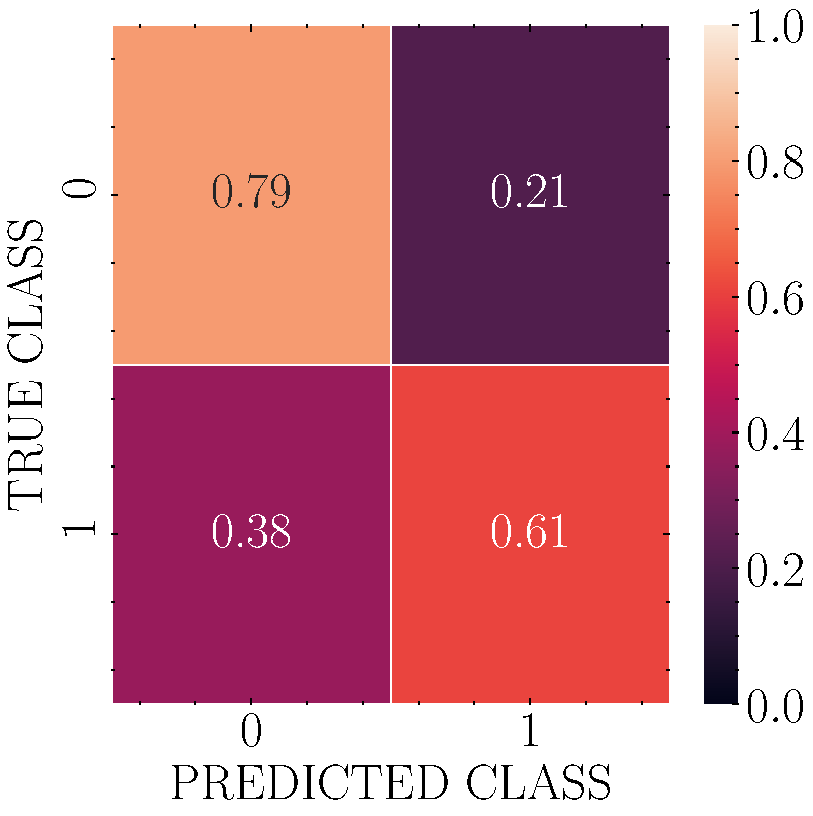
\includegraphics[width=1.8in]{../results/ex1/conf_mtx_QD_ML_dataset_P1a_size_10.pdf}
       \caption{QDA, size $10$.}
       \label{fig:QDA_P1a_10}
    \end{subfigure}
\quad \quad
    \begin{subfigure}[!htbp]{0.24\textwidth}
       \centering
       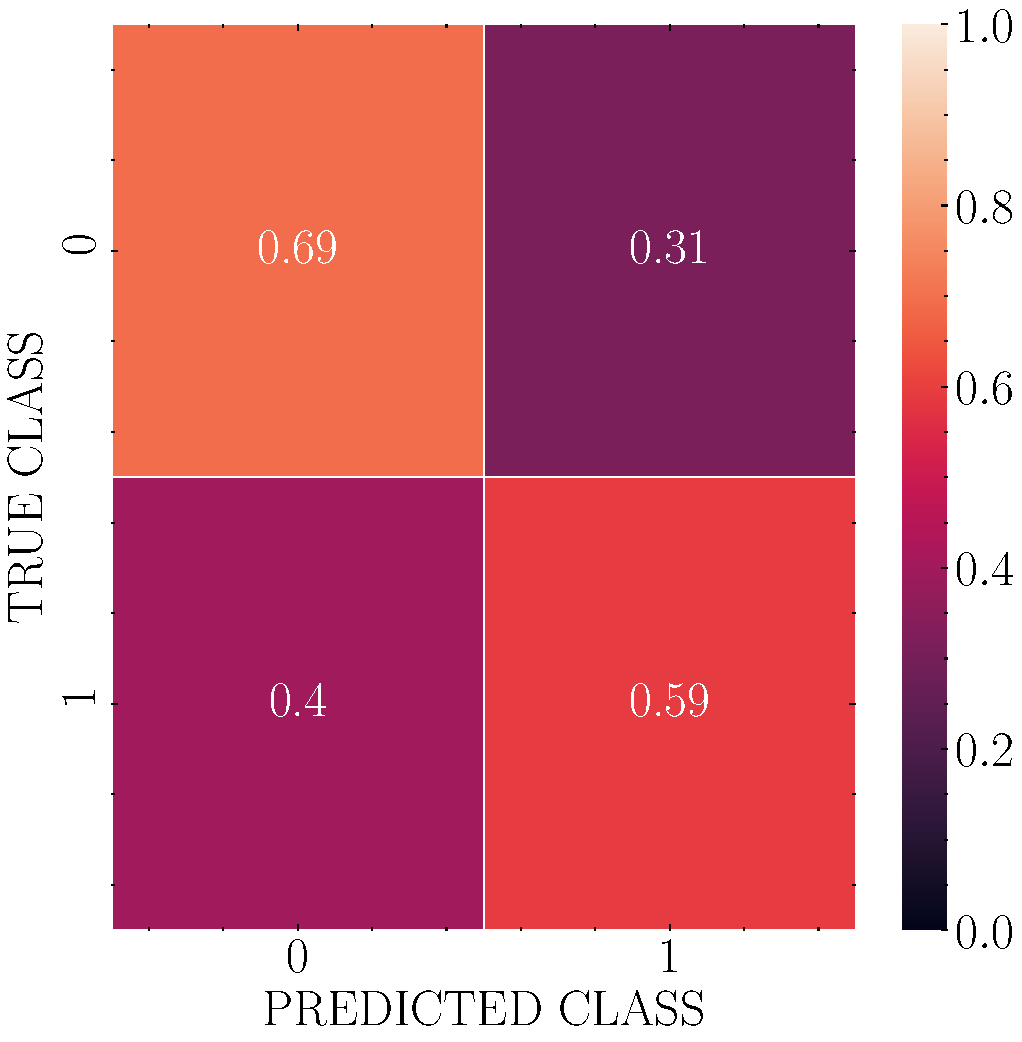
\includegraphics[width=1.8in]{../results/ex1/conf_mtx_KNN_dataset_P1a_size_10.pdf}
       \caption{KNN, size $10$.}
       \label{fig:KNN_P1a_10}
    \end{subfigure}
\quad \quad
    \begin{subfigure}[!htbp]{0.24\textwidth}
       \centering
       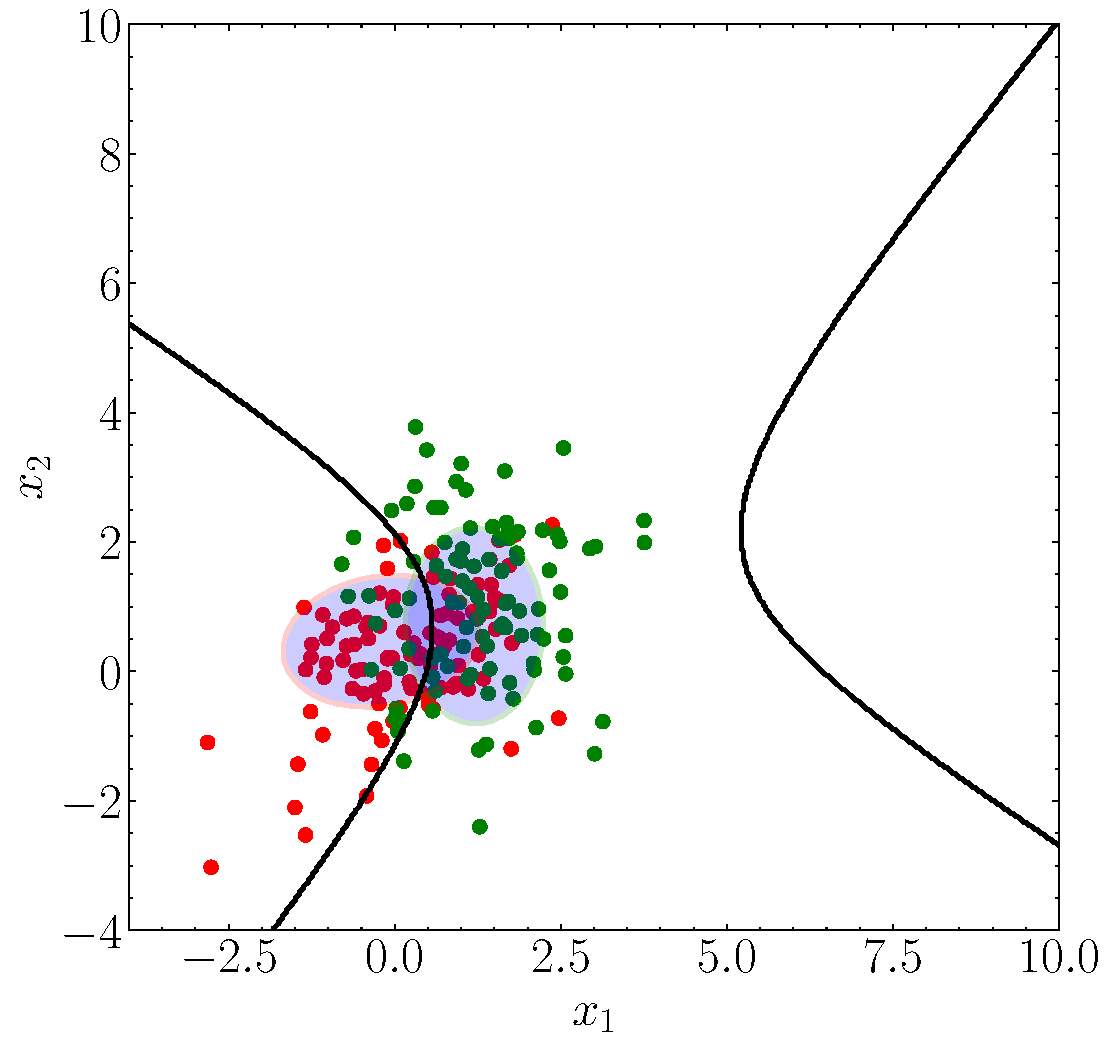
\includegraphics[width=1.8in]{../results/ex1/samples_QD_ML_dataset_P1a_size_10.pdf}
       \caption{Samples, size $10$.}
       \label{fig:DF_P1a_10}
    \end{subfigure}
    
\quad \quad 
    \begin{subfigure}[!htbp]{0.24\textwidth}
       \centering
       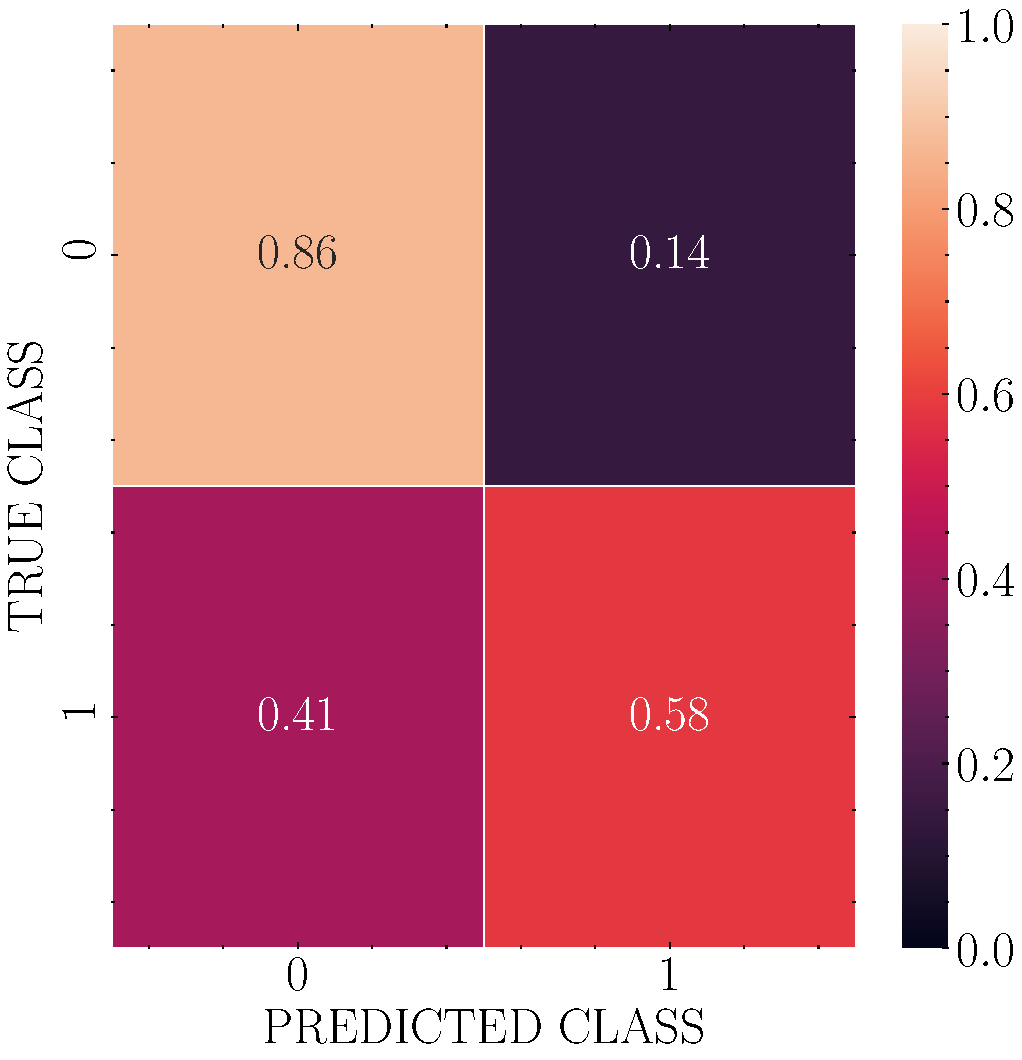
\includegraphics[width=1.8in]{../results/ex1/conf_mtx_QD_ML_dataset_P1a_size_25.pdf}
       \caption{QDA, size $25$.}
       \label{fig:QDA_P1a_25}
    \end{subfigure}
\quad \quad 
    \begin{subfigure}[!htbp]{0.24\textwidth}
       \centering
       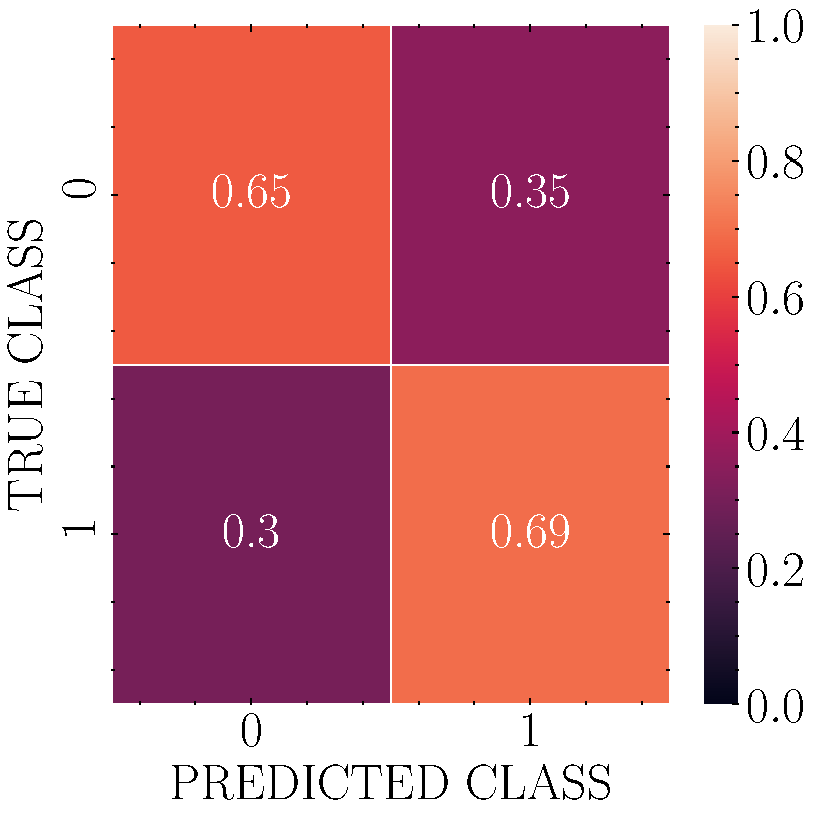
\includegraphics[width=1.8in]{../results/ex1/conf_mtx_KNN_dataset_P1a_size_25.pdf}
       \caption{KNN, size $25$.}
       \label{fig:KNN_P1a_25}
    \end{subfigure}
\quad \quad
    \begin{subfigure}[!htbp]{0.24\textwidth}
       \centering
       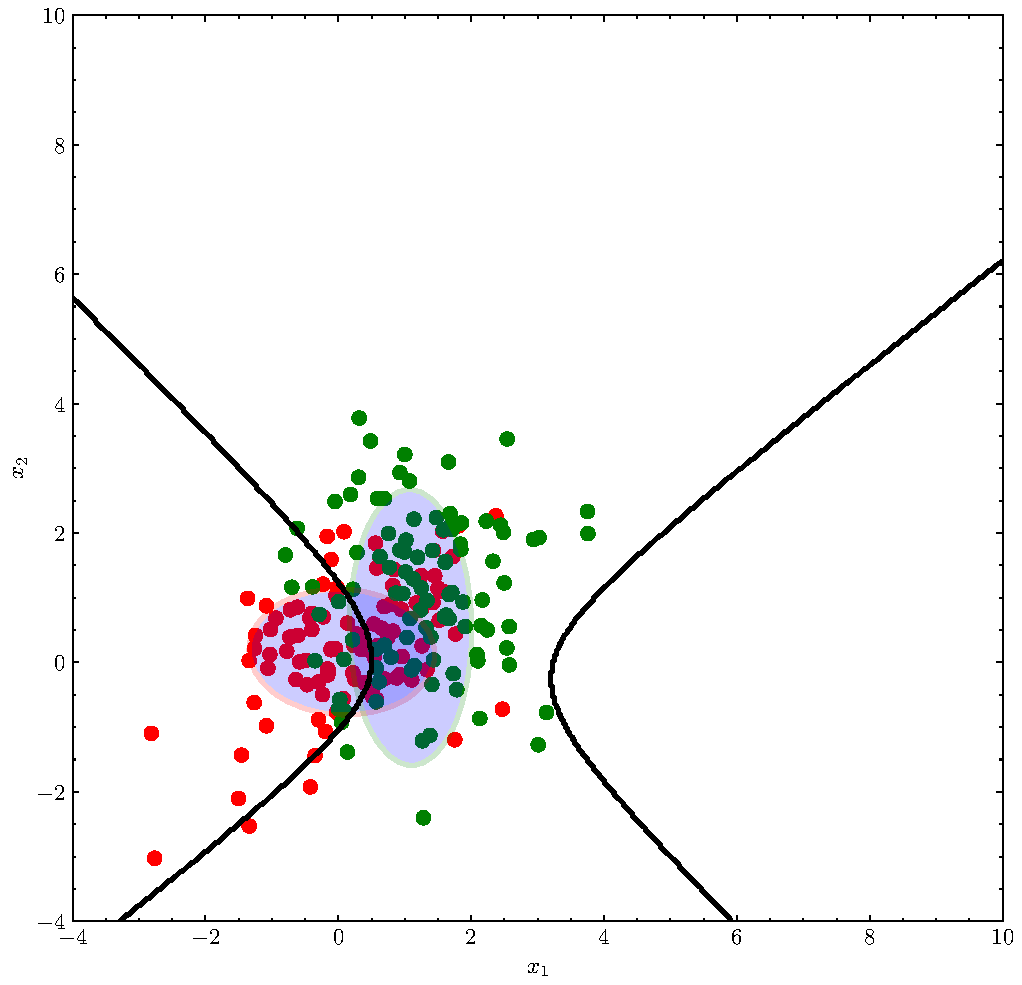
\includegraphics[width=1.8in]{../results/ex1/samples_QD_ML_dataset_P1a_size_25.pdf}
       \caption{Samples, size $25$.}
       \label{fig:DF_P1a_25}
    \end{subfigure}
    
\quad \quad
    \begin{subfigure}[!htbp]{0.24\textwidth}
       \centering
       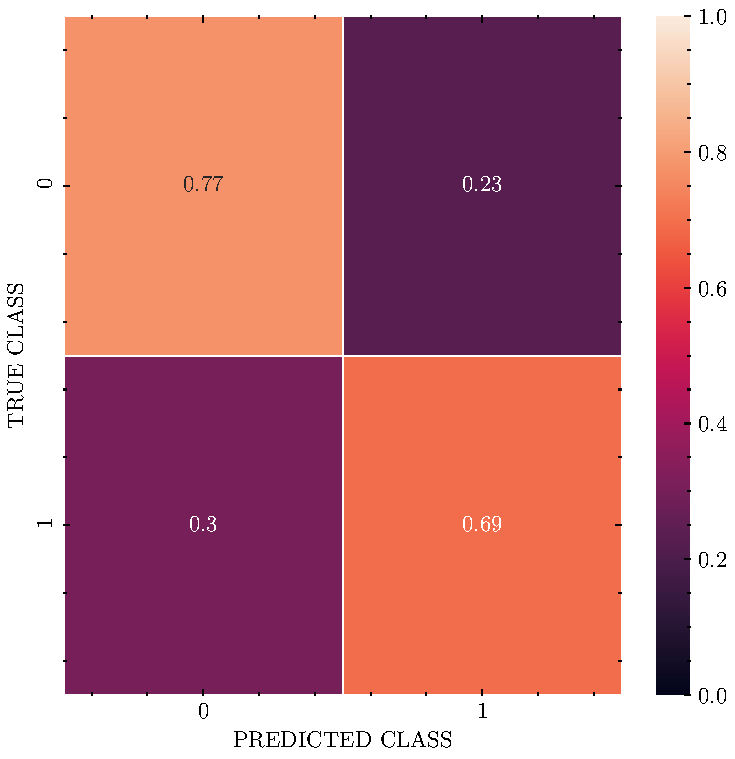
\includegraphics[width=1.8in]{../results/ex1/conf_mtx_QD_ML_dataset_P1a_size_75.pdf}
       \caption{QDA, size $75$.}
       \label{fig:QDA_P1a_75}
    \end{subfigure}
\quad \quad
    \begin{subfigure}[!htbp]{0.24\textwidth}
       \centering
       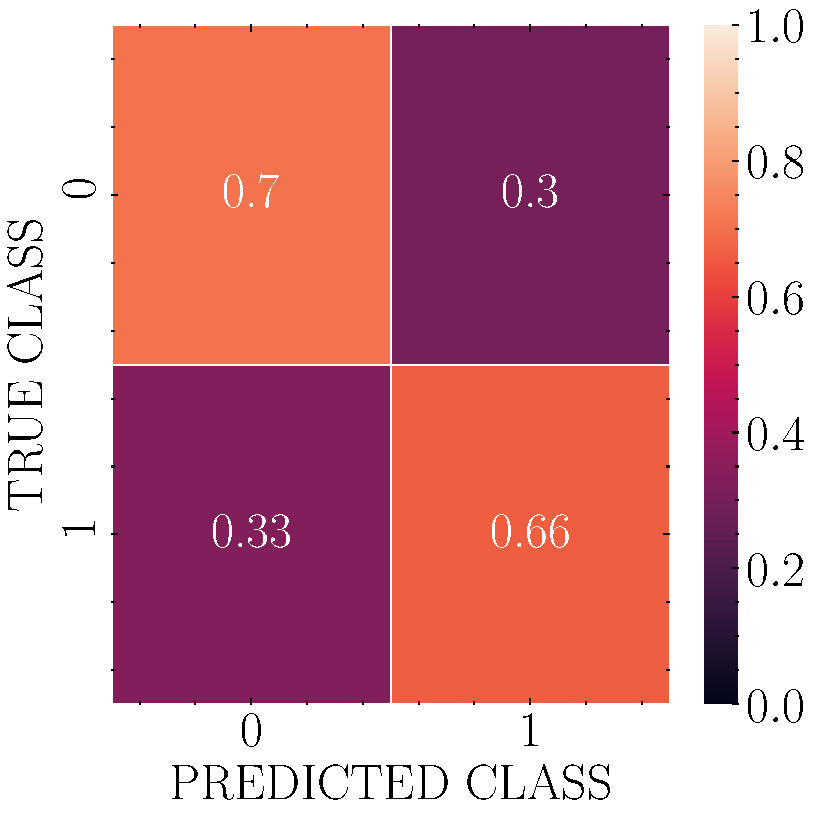
\includegraphics[width=1.8in]{../results/ex1/conf_mtx_KNN_dataset_P1a_size_75.pdf}
       \caption{KNN, size $75$.}
       \label{fig:KNN_P1a_75}
    \end{subfigure}
\quad \quad
    \begin{subfigure}[!htbp]{0.24\textwidth}
       \centering
       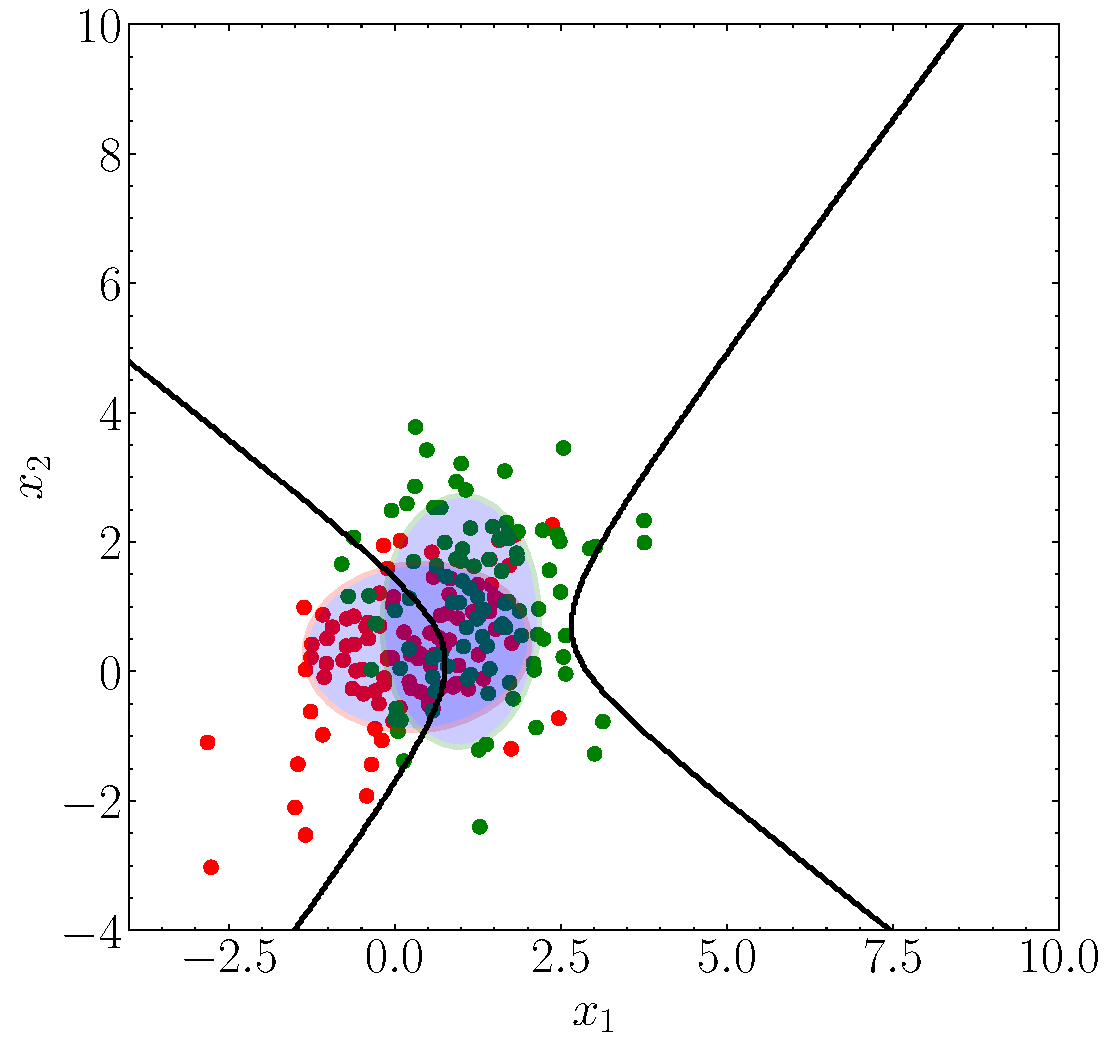
\includegraphics[width=1.8in]{../results/ex1/samples_QD_ML_dataset_P1a_size_75.pdf}
       \caption{Samples, size $75$.}
       \label{fig:DF_P1a_75}
    \end{subfigure}
    
\quad \quad
    \begin{subfigure}[!htbp]{0.24\textwidth}
       \centering
       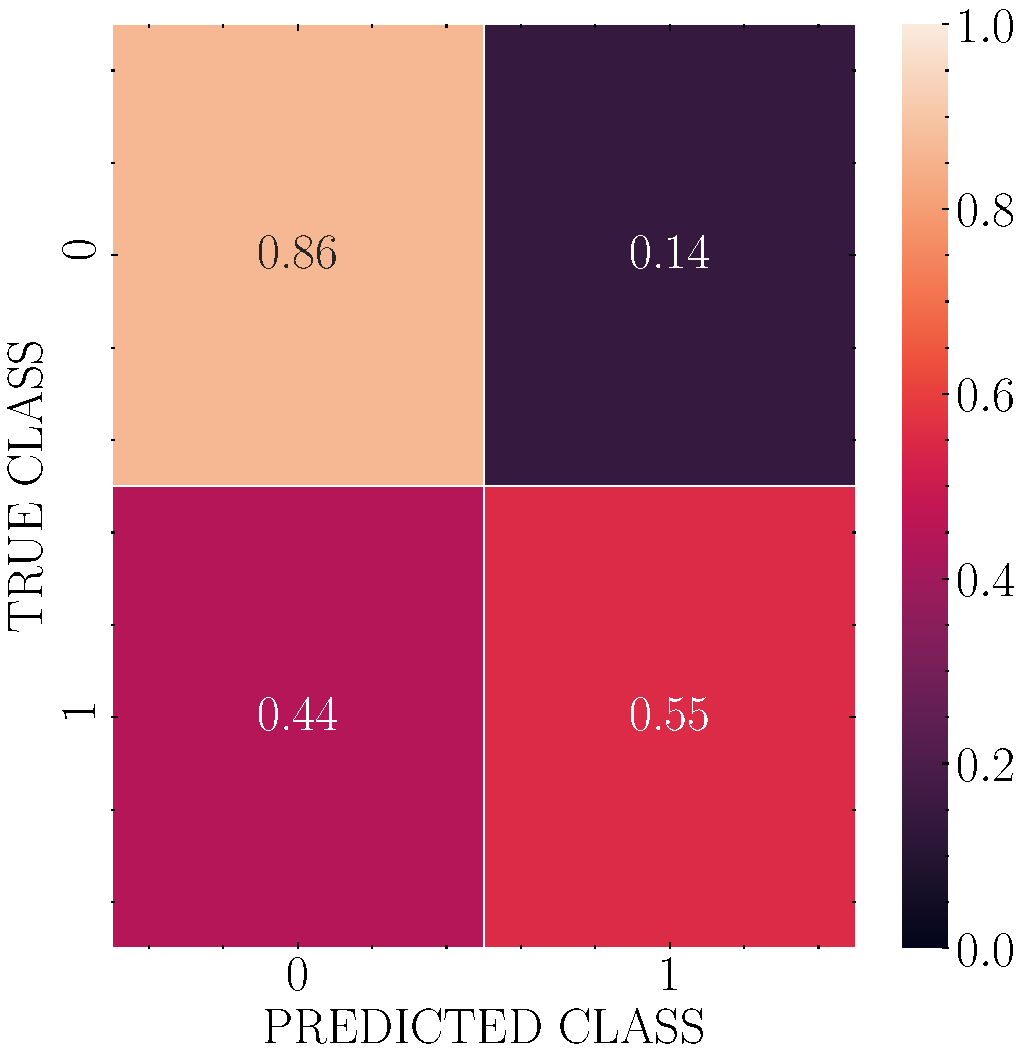
\includegraphics[width=1.8in]{../results/ex1/conf_mtx_QD_ML_dataset_P1a_size_199.pdf}
       \caption{QDA, size $199$.}
       \label{fig:QDA_P1a_199}
    \end{subfigure}
\quad \quad 
    \begin{subfigure}[!htbp]{0.24\textwidth}
       \centering
       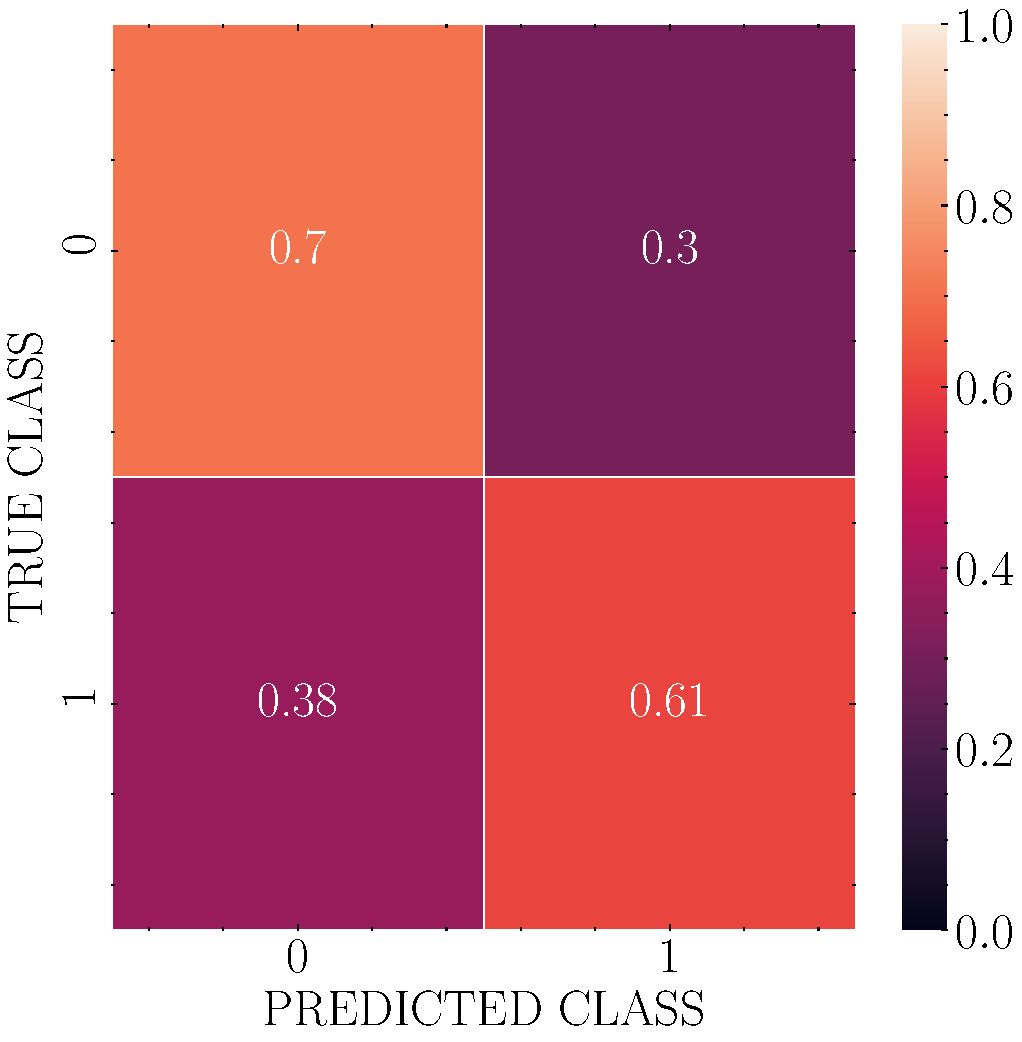
\includegraphics[width=1.8in]{../results/ex1/conf_mtx_KNN_dataset_P1a_size_199.pdf}
       \caption{KNN, size $199$.}
       \label{fig:KNN_P1a_199}
    \end{subfigure}
\quad \quad
    \begin{subfigure}[!htbp]{0.24\textwidth}
       \centering
       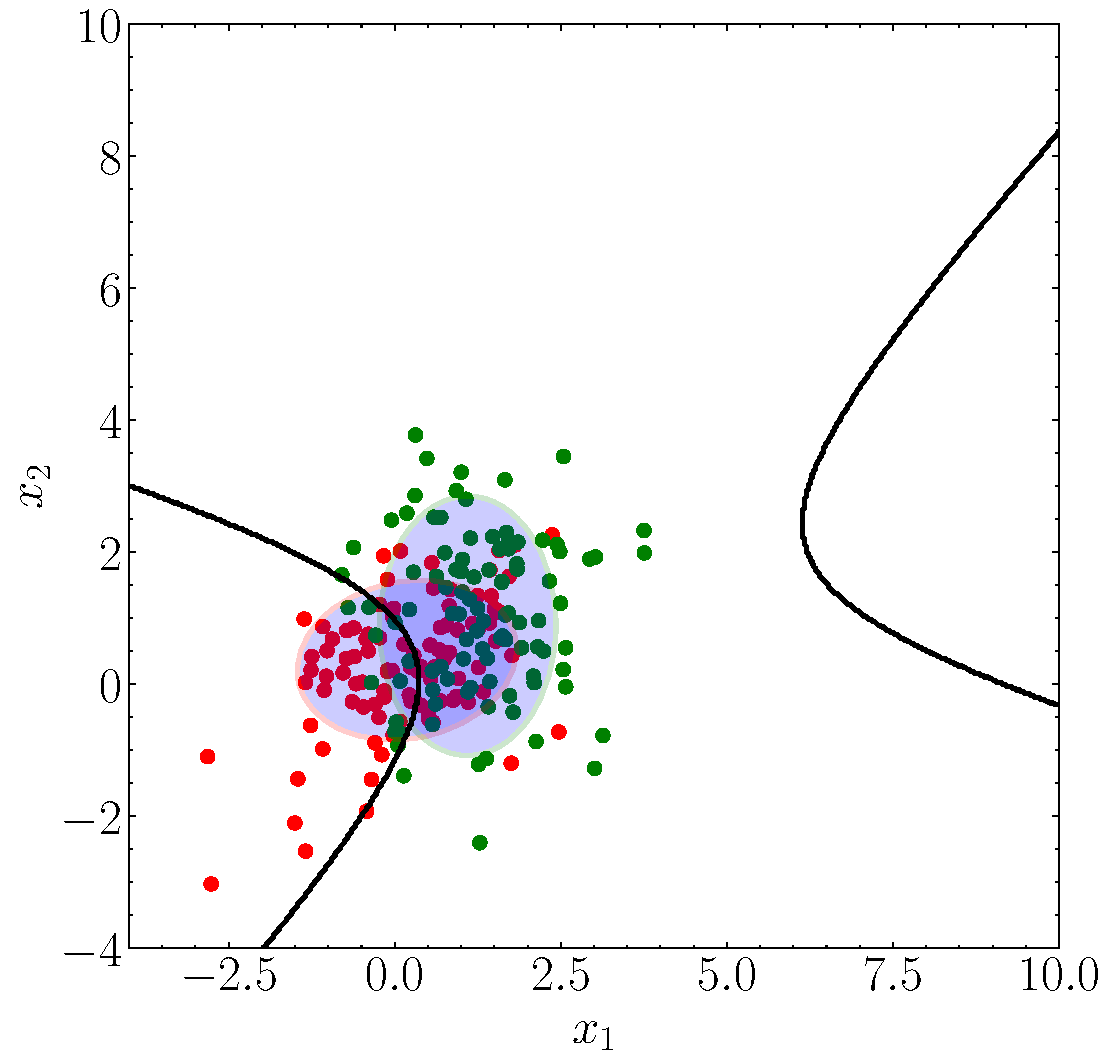
\includegraphics[width=1.8in]{../results/ex1/samples_QD_ML_dataset_P1a_size_199.pdf}
       \caption{Samples, size $199$.}
       \label{fig:DF_P1a_199}
    \end{subfigure}

\caption{Bayes classifier and Nearest neighbour classification on P1a dataset.}
\label{fig:ex11P1a}
\end{figure}

\underline {\it \bfseries Inferences on P1b}: The class means are $\bmu_{0} = [0 \; 0]^{\TT}$ and $\bmu_{1} = [3 \; 3]^{\TT}$, and the covariances are in the same order. The class distributions are farther apart, i.e., the discriminability is higher than in P1a. This is seen with the training samples from each class barely overlapping into the other class. Within this setting, the classifiers trained with training sizes $10$, $25$, $75$, and $199$ on the average show, show an increasing trend in test accuracy. The nearest-neighbour classifier performs comparably to the Bayes' classifier. In no case, the error in classification using nearest-neighbour classifier exceeds twice the error in the Bayes' classifier. With increasing size of the training set, the learnt Gaussians is observed to learn ``better'', i.e., the means and covariances are closer to the true values. \\

\begin{figure}[!htbp]
\centering
\quad \quad
    \begin{subfigure}[!htbp]{0.24\textwidth}
       \centering
       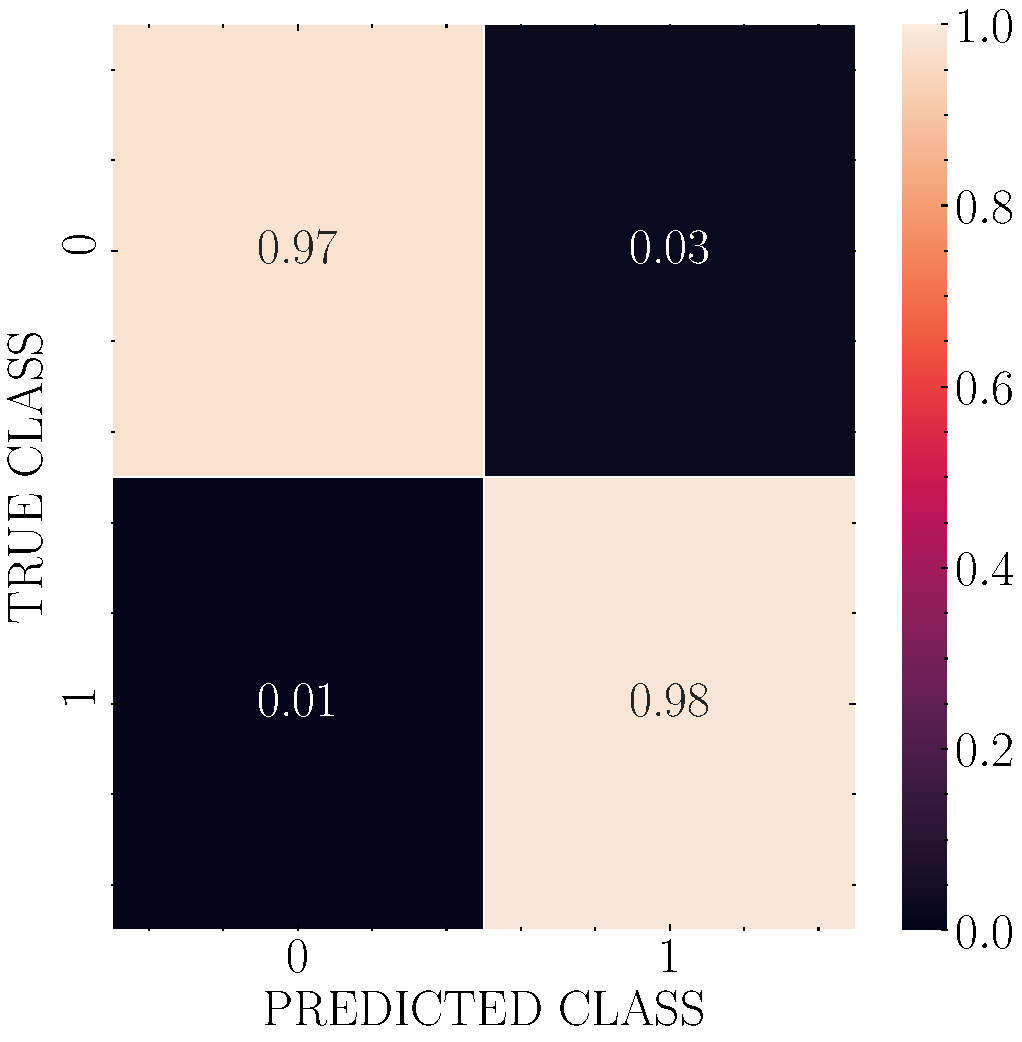
\includegraphics[width=1.8in]{../results/ex1/conf_mtx_QD_ML_dataset_P1b_size_10.pdf}
       \caption{QDA, size $10$.}
       \label{fig:QDA_P1b_10}
    \end{subfigure}
\quad \quad
    \begin{subfigure}[!htbp]{0.24\textwidth}
       \centering
       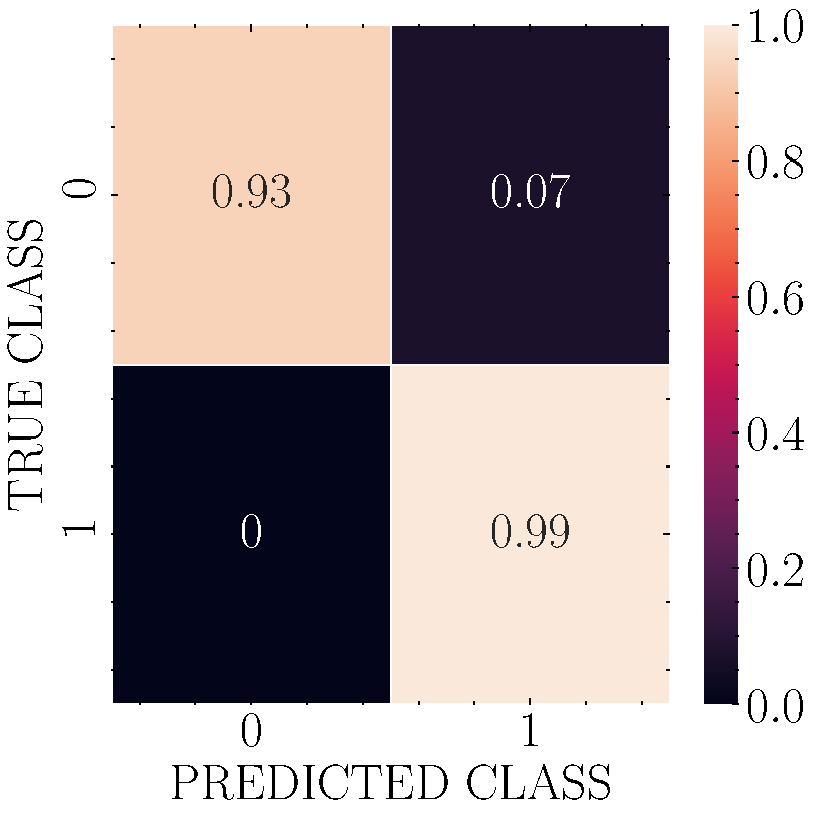
\includegraphics[width=1.8in]{../results/ex1/conf_mtx_KNN_dataset_P1b_size_10.pdf}
       \caption{KNN, size $10$.}
       \label{fig:KNN_P1b_10}
    \end{subfigure}
\quad \quad
    \begin{subfigure}[!htbp]{0.24\textwidth}
       \centering
       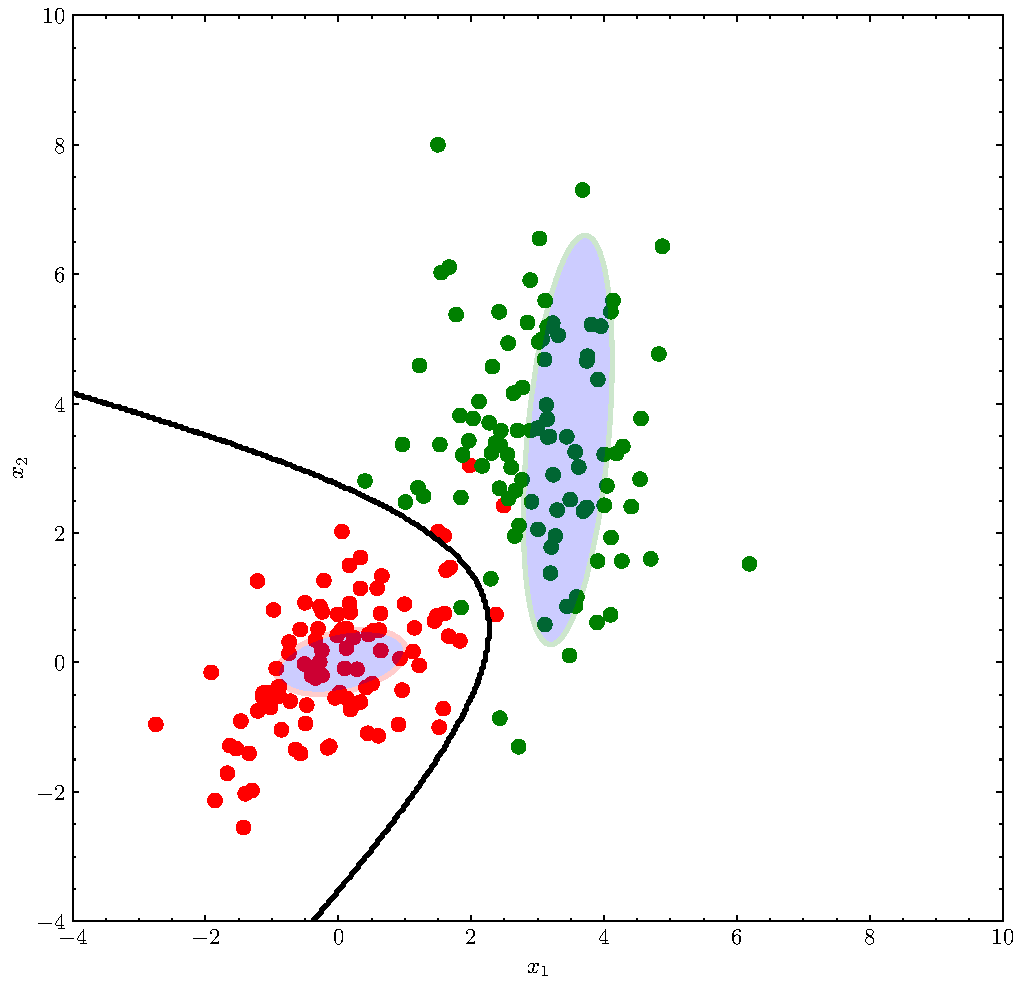
\includegraphics[width=1.8in]{../results/ex1/samples_QD_ML_dataset_P1b_size_10.pdf}
       \caption{Samples, size $10$.}
       \label{fig:KNN_P1b_10}
    \end{subfigure}
    
\quad \quad 
    \begin{subfigure}[!htbp]{0.24\textwidth}
       \centering
       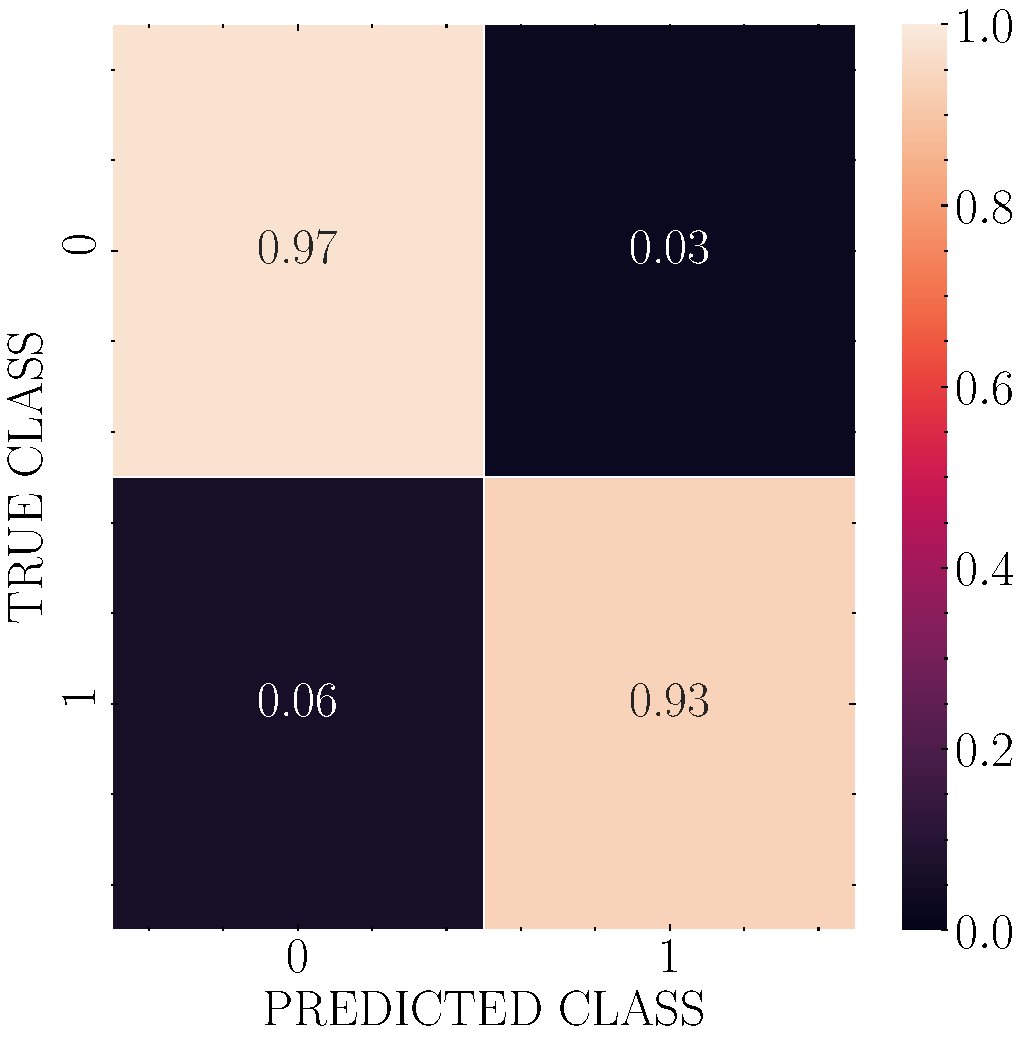
\includegraphics[width=1.8in]{../results/ex1/conf_mtx_QD_ML_dataset_P1b_size_25.pdf}
       \caption{QDA, size $25$.}
       \label{fig:KNN_P1b_25}
    \end{subfigure}
\quad \quad
    \begin{subfigure}[!htbp]{0.24\textwidth}
       \centering
       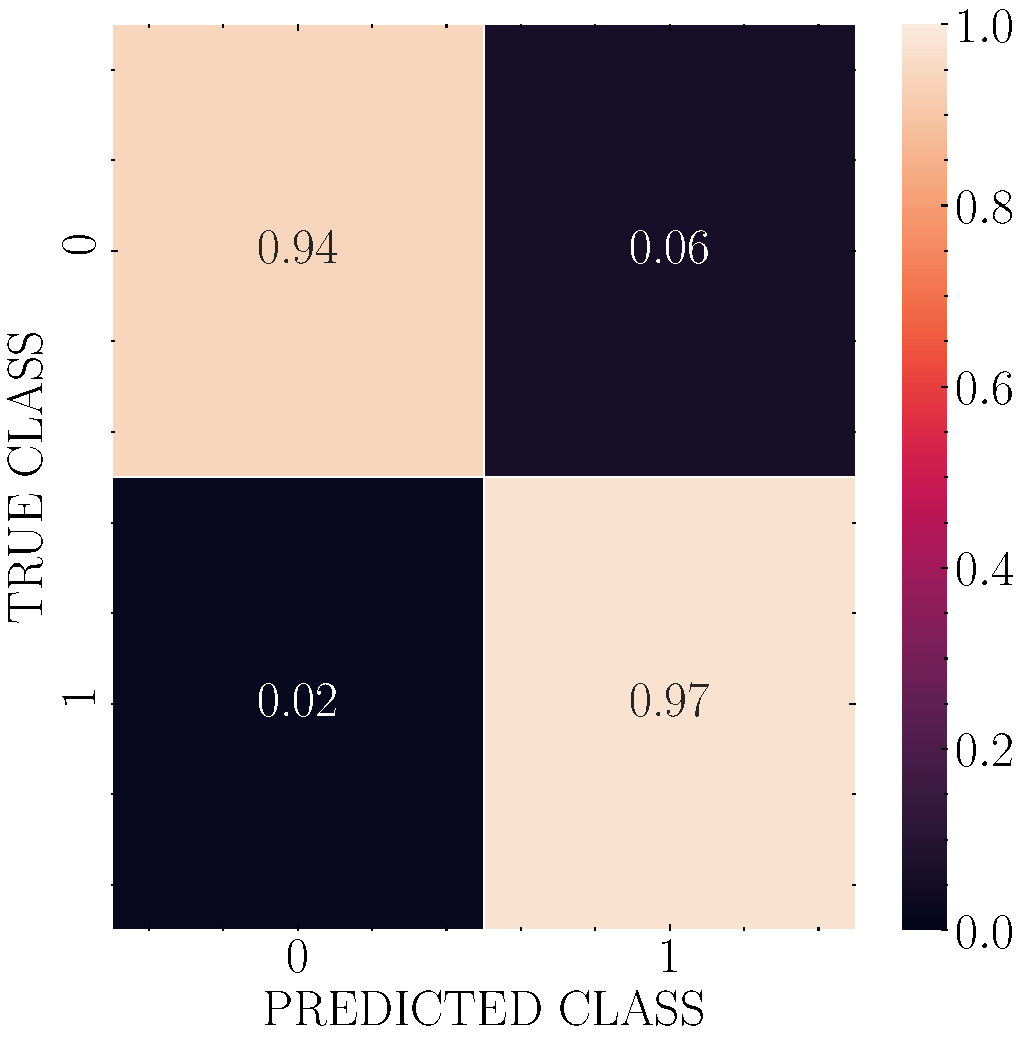
\includegraphics[width=1.8in]{../results/ex1/conf_mtx_KNN_dataset_P1b_size_25.pdf}
       \caption{KNN, size $25$.}
       \label{fig:KNN_P1b_25}
    \end{subfigure}
\quad
    \begin{subfigure}[!htbp]{0.24\textwidth}
       \centering
       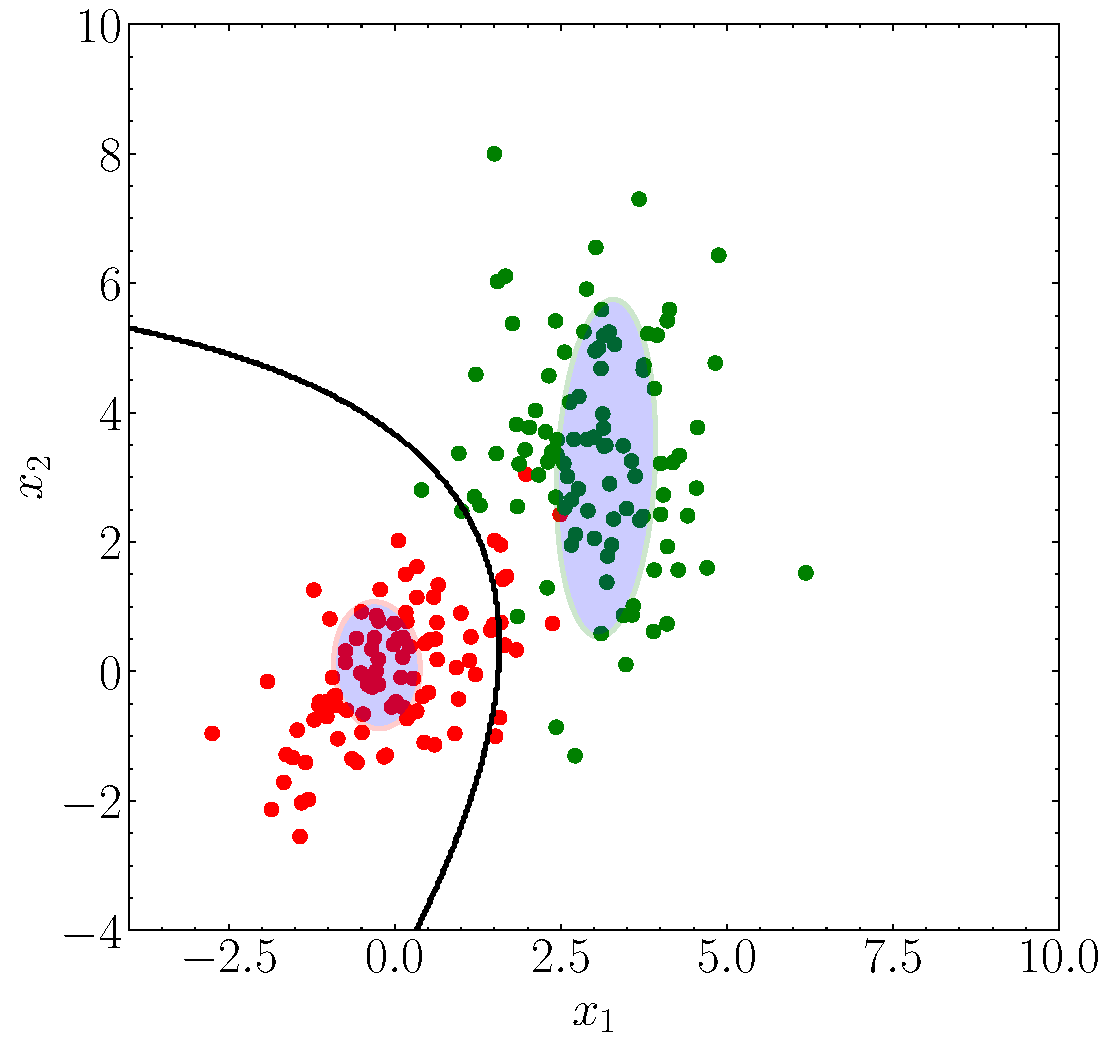
\includegraphics[width=1.8in]{../results/ex1/samples_QD_ML_dataset_P1b_size_25.pdf}
       \caption{Samples, size $25$.}
       \label{fig:KNN_P1b_25}
    \end{subfigure}
    
\quad \quad 
    \begin{subfigure}[!htbp]{0.24\textwidth}
       \centering
       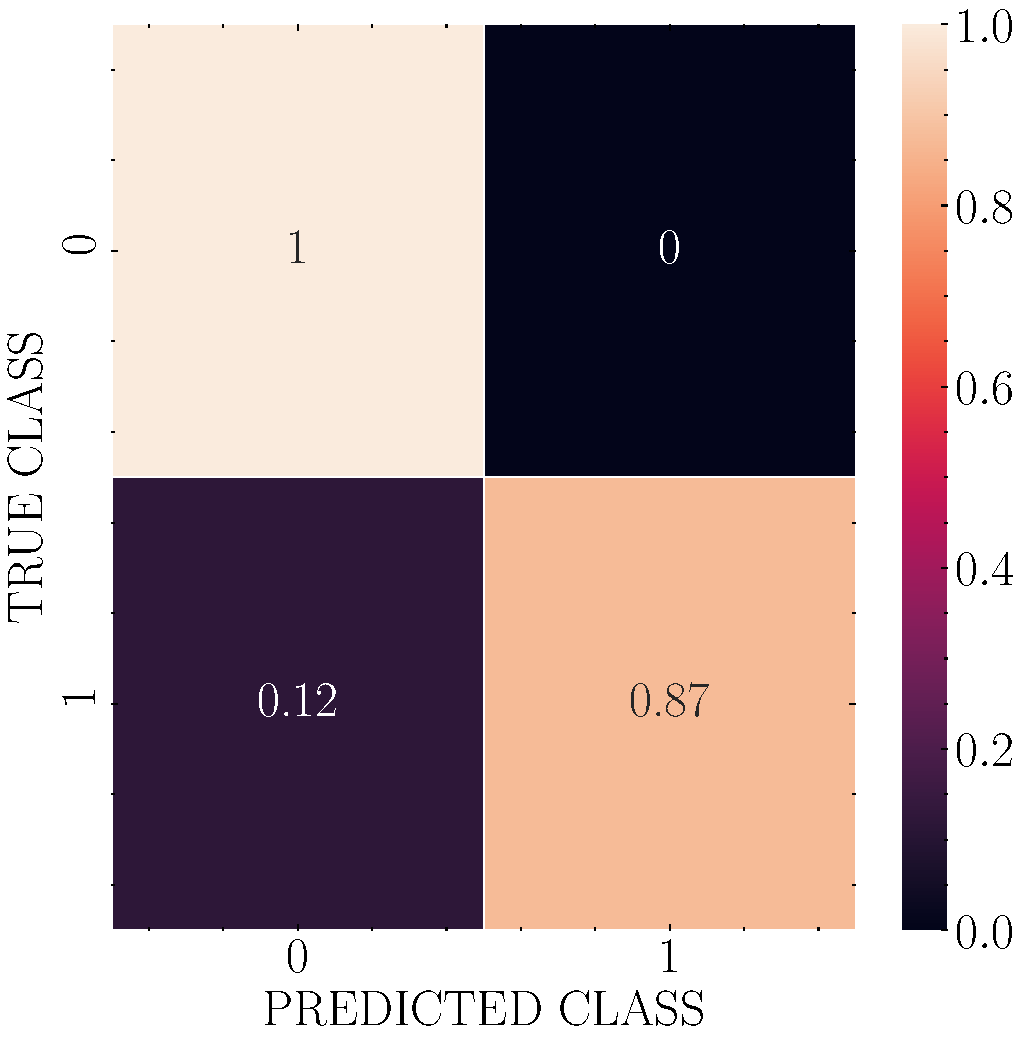
\includegraphics[width=1.8in]{../results/ex1/conf_mtx_QD_ML_dataset_P1b_size_75.pdf}
       \caption{QDA, size $75$.}
       \label{fig:KNN_P1b_75}
    \end{subfigure}
\quad \quad   
    \begin{subfigure}[!htbp]{0.24\textwidth}
       \centering
       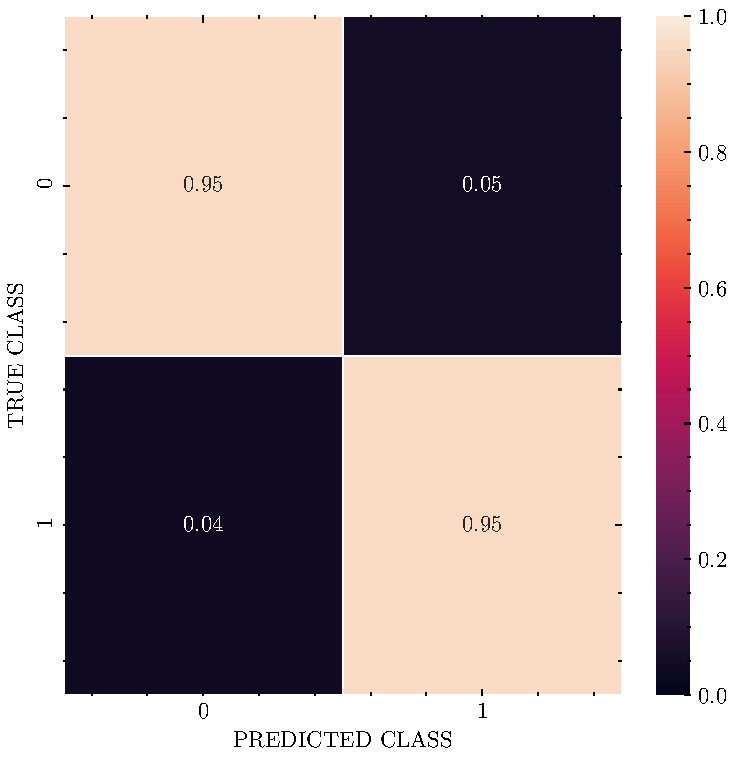
\includegraphics[width=1.8in]{../results/ex1/conf_mtx_KNN_dataset_P1b_size_75.pdf}
       \caption{KNN, size $75$.}
       \label{fig:KNN_P1b_75}
    \end{subfigure}
\quad \quad
    \begin{subfigure}[!htbp]{0.24\textwidth}
       \centering
       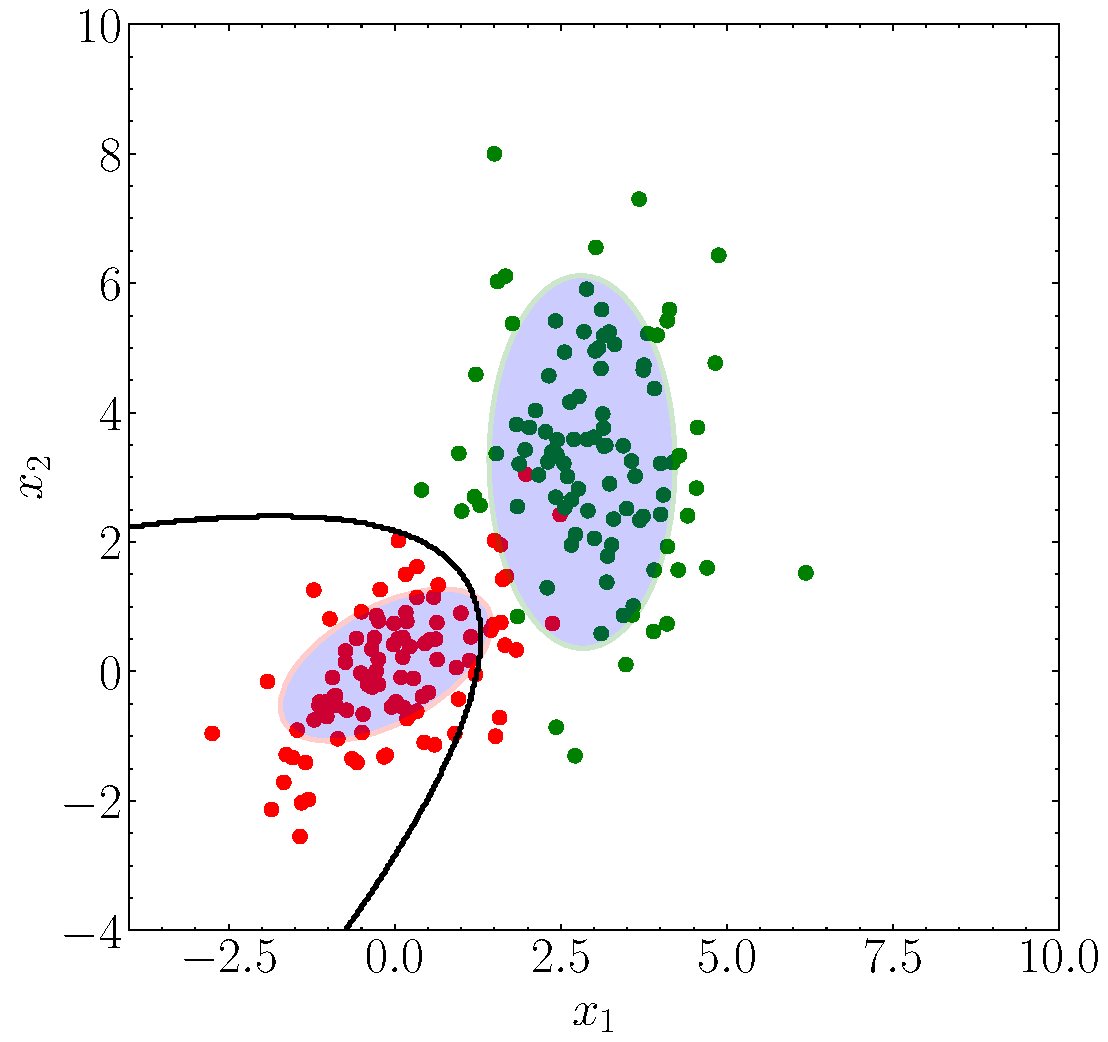
\includegraphics[width=1.8in]{../results/ex1/samples_QD_ML_dataset_P1b_size_75.pdf}
       \caption{Samples, size $75$.}
       \label{fig:KNN_P1b_75}
    \end{subfigure}
    
\quad \quad
    \begin{subfigure}[!htbp]{0.24\textwidth}
       \centering
       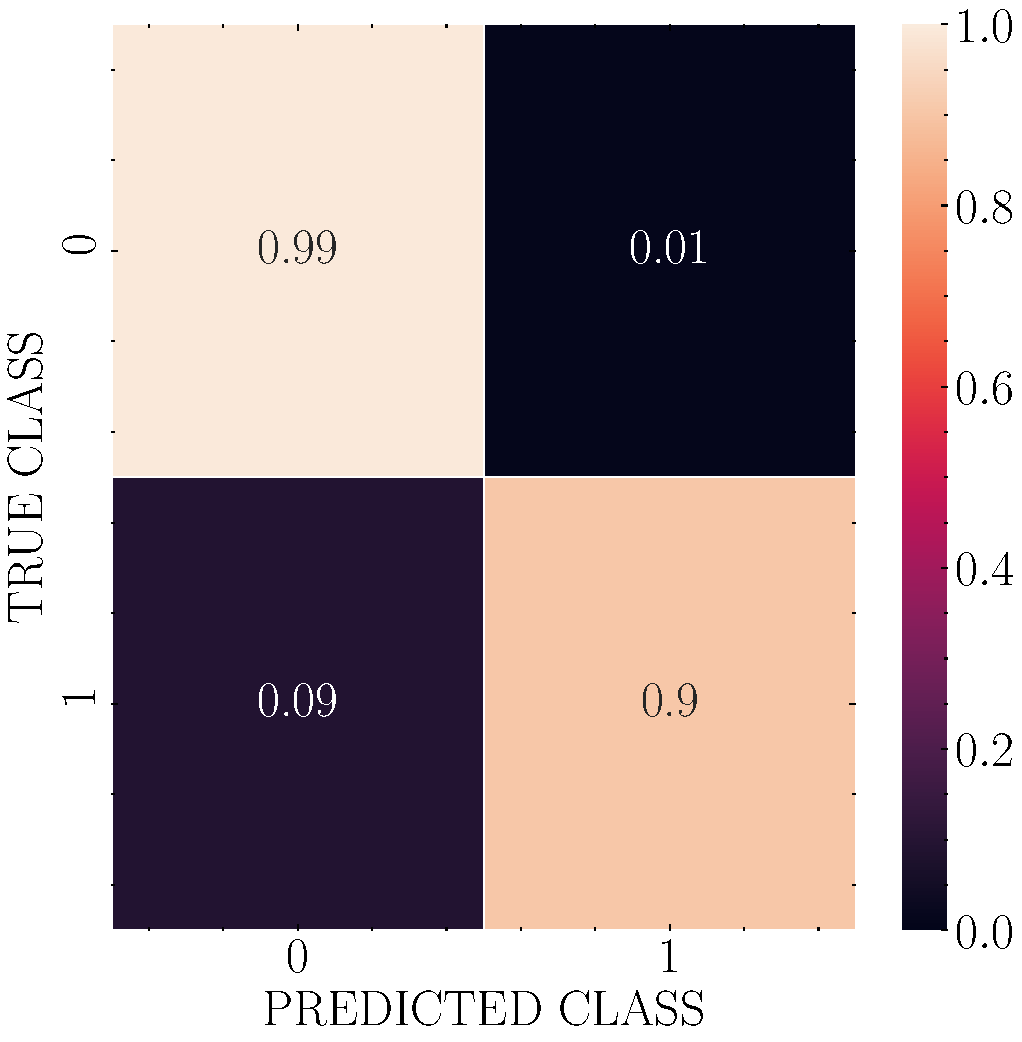
\includegraphics[width=1.8in]{../results/ex1/conf_mtx_QD_ML_dataset_P1b_size_199.pdf}
       \caption{QDA, size $199$.}
       \label{fig:KNN_P1b_199}
    \end{subfigure}
\quad \quad
    \begin{subfigure}[!htbp]{0.24\textwidth}
       \centering
       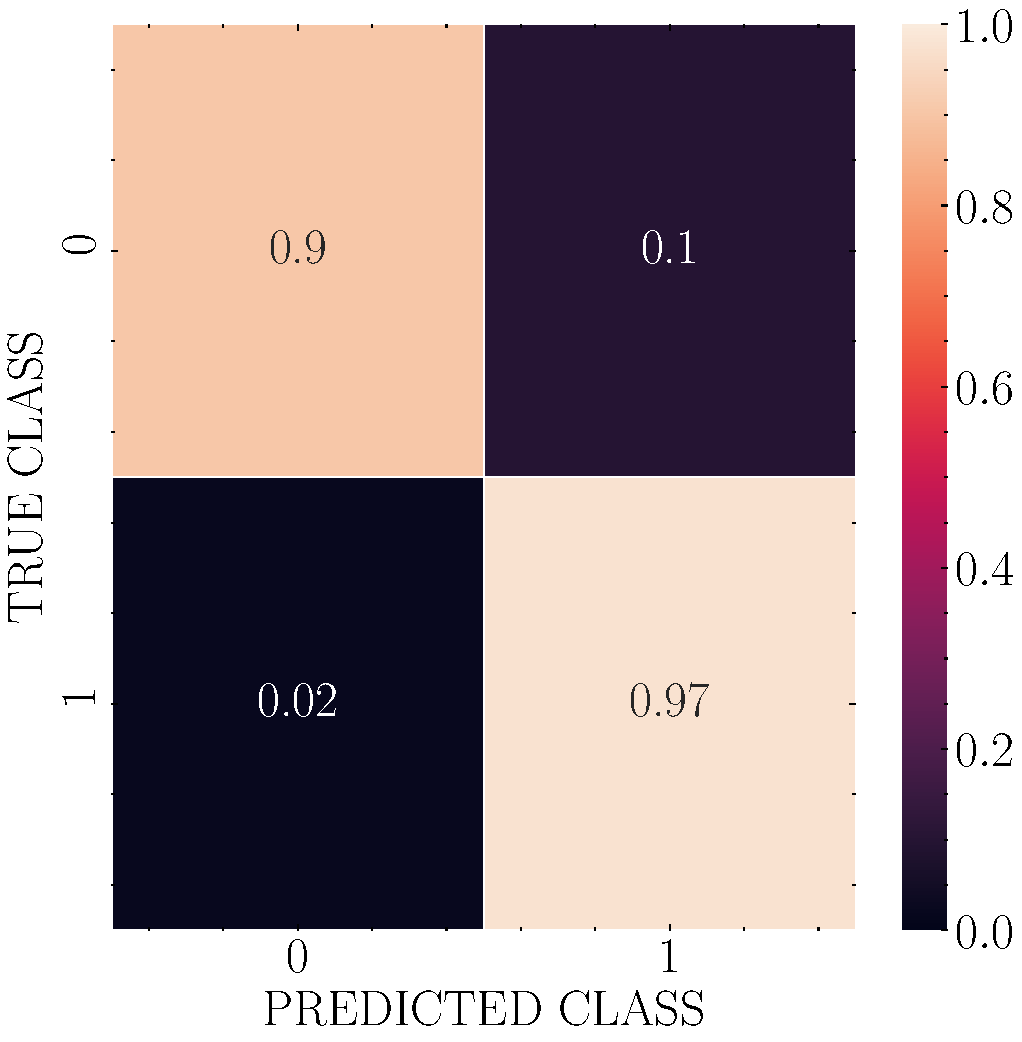
\includegraphics[width=1.8in]{../results/ex1/conf_mtx_KNN_dataset_P1b_size_199.pdf}
       \caption{KNN, size $199$.}
       \label{fig:KNN_P1b_199}
    \end{subfigure}
\quad \quad
    \begin{subfigure}[!htbp]{0.24\textwidth}
       \centering
       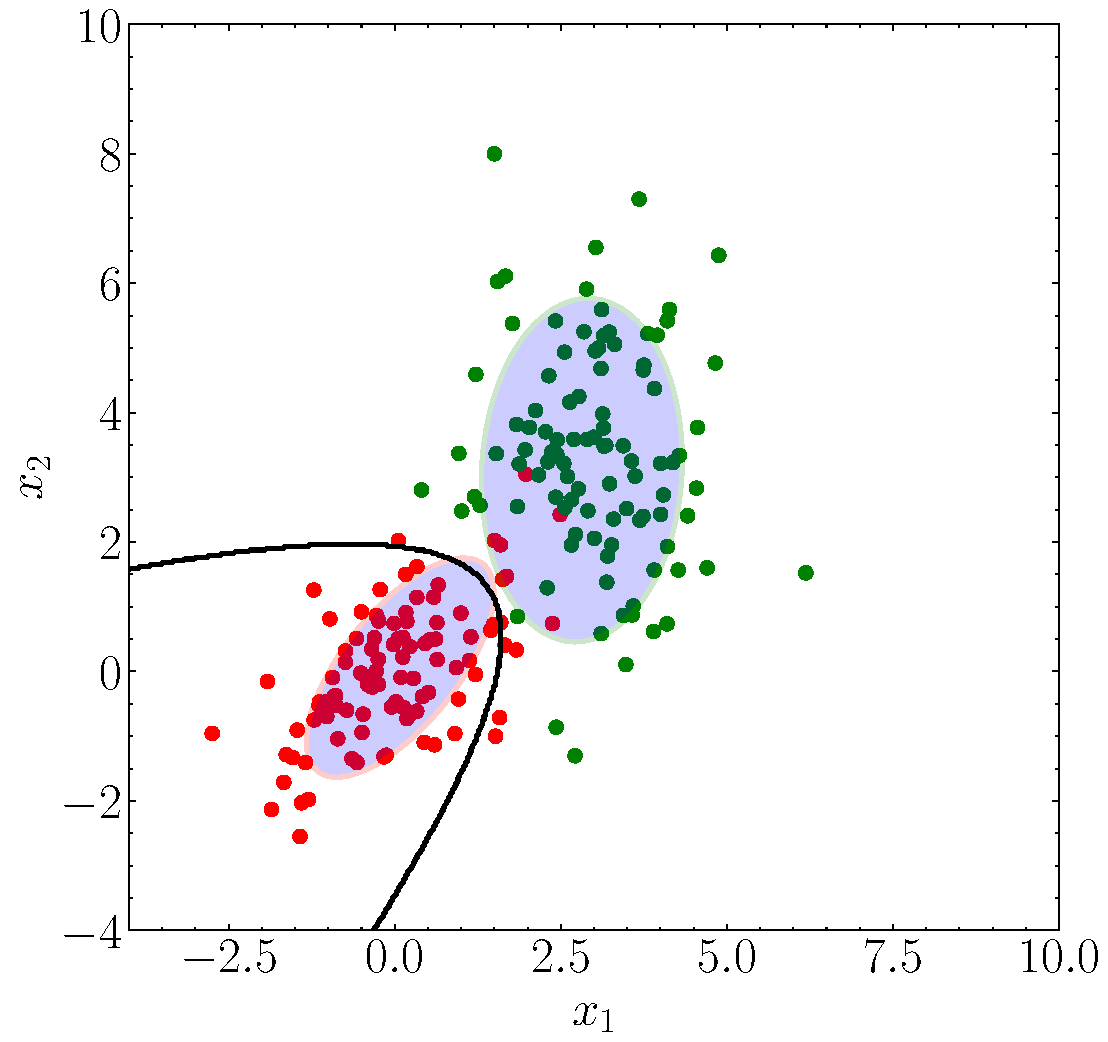
\includegraphics[width=1.8in]{../results/ex1/samples_QD_ML_dataset_P1b_size_199.pdf}
       \caption{Samples, size $199$.}
       \label{fig:KNN_P1b_199}
    \end{subfigure}

\caption{Bayes classifier and Nearest neighbour classification on P1b dataset.}
\label{fig:ex11P1b}
\end{figure}

\begin{figure}[!htbp]
\centering
\quad \quad
    \begin{subfigure}[!htbp]{0.24\textwidth}
       \centering
       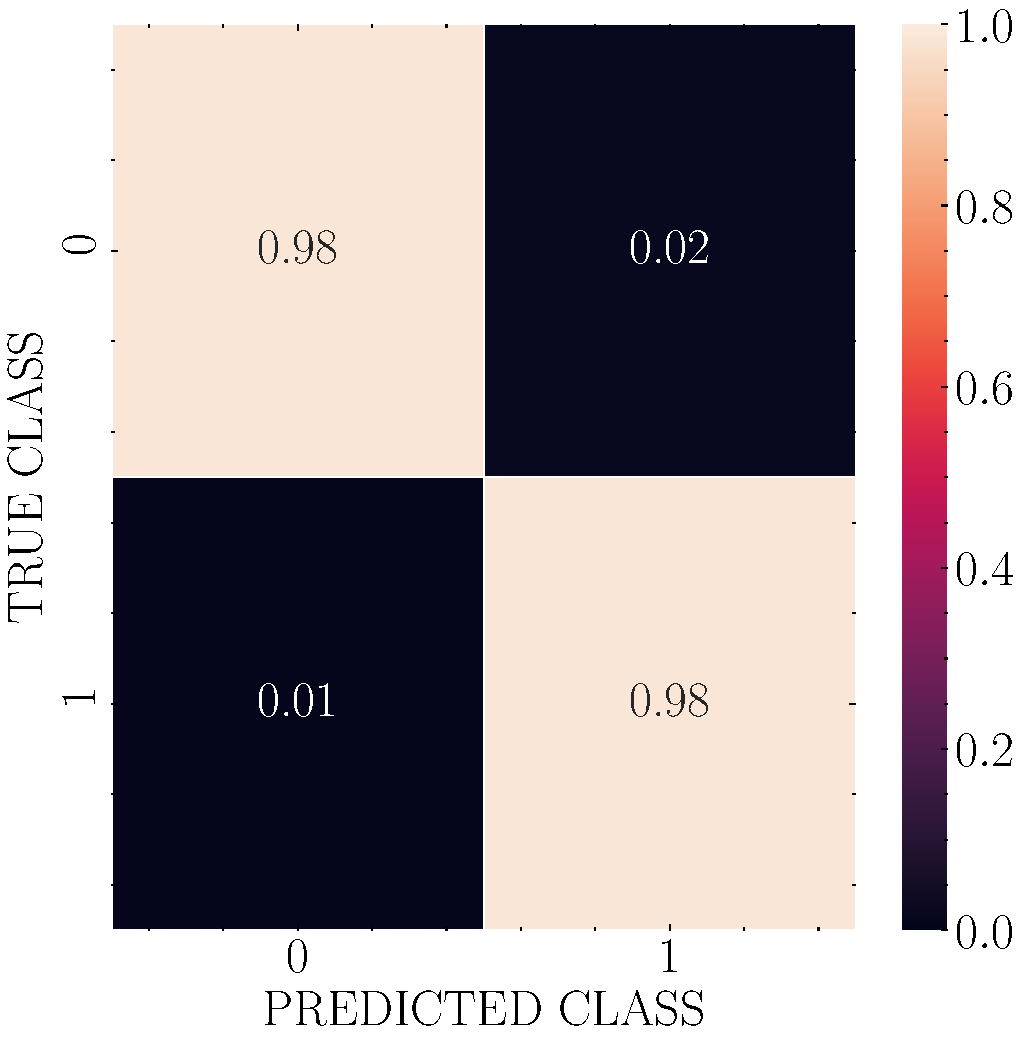
\includegraphics[width=1.8in]{../results/ex1/conf_mtx_QD_ML_dataset_P1c_size_10.pdf}
       \caption{QDA, size $10$.}
       \label{fig:QDA_P1c_10}
    \end{subfigure}
\quad \quad
    \begin{subfigure}[!htbp]{0.24\textwidth}
       \centering
       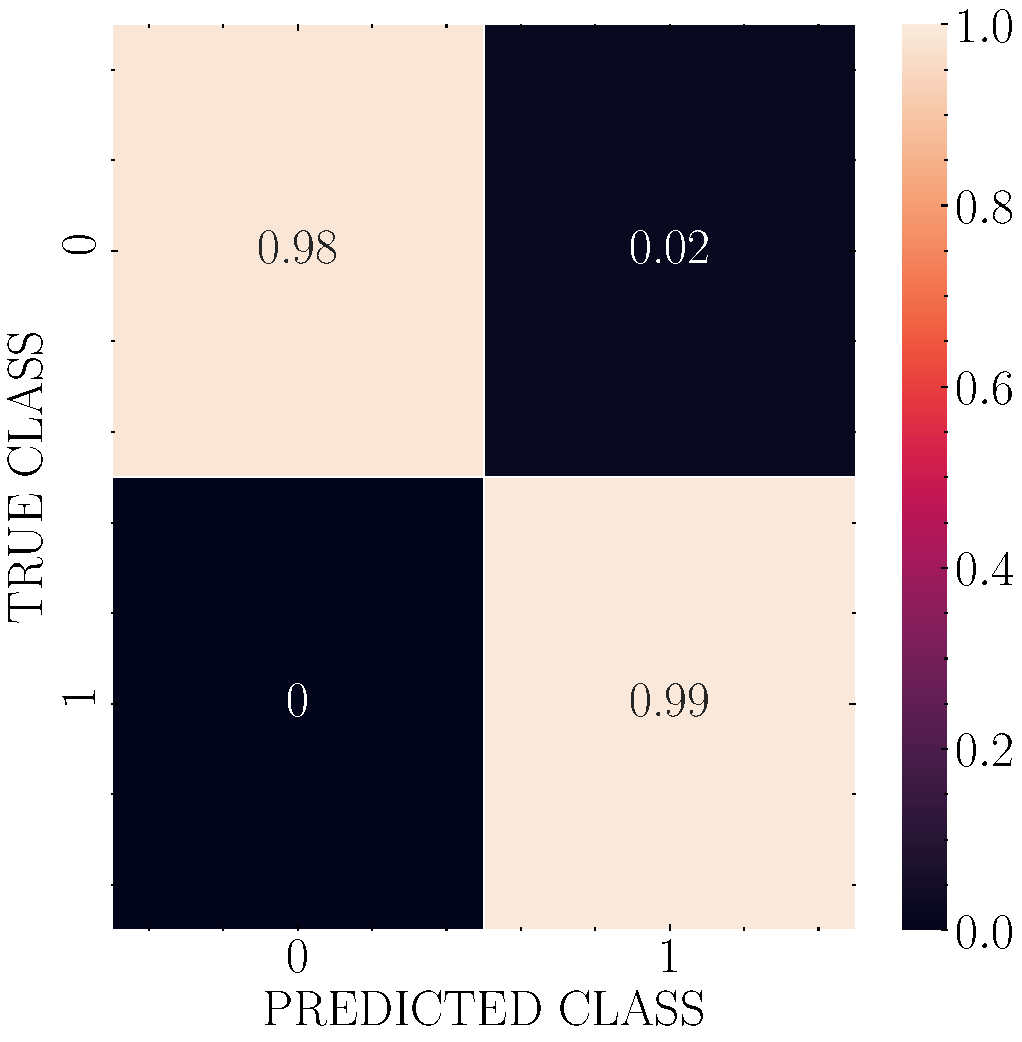
\includegraphics[width=1.8in]{../results/ex1/conf_mtx_KNN_dataset_P1c_size_10.pdf}
       \caption{KNN, size $10$.}
       \label{fig:KNN_P1c_10}
    \end{subfigure}
\quad \quad
    \begin{subfigure}[!htbp]{0.24\textwidth}
       \centering
       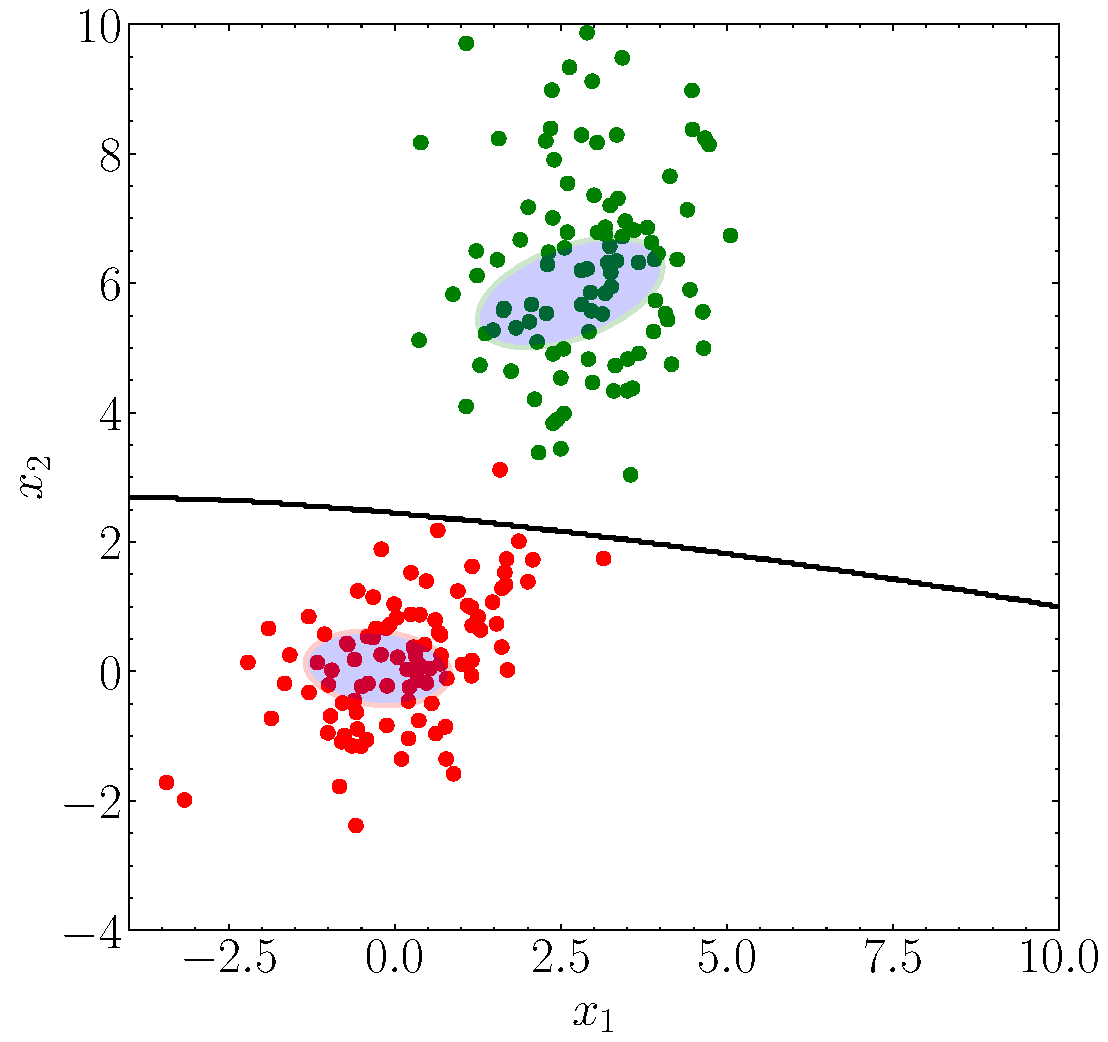
\includegraphics[width=1.8in]{../results/ex1/samples_QD_ML_dataset_P1c_size_10.pdf}
       \caption{Samples, size $10$.}
       \label{fig:KNN_P1c_10}
    \end{subfigure}
    
\quad \quad   
    \begin{subfigure}[!htbp]{0.24\textwidth}
       \centering
       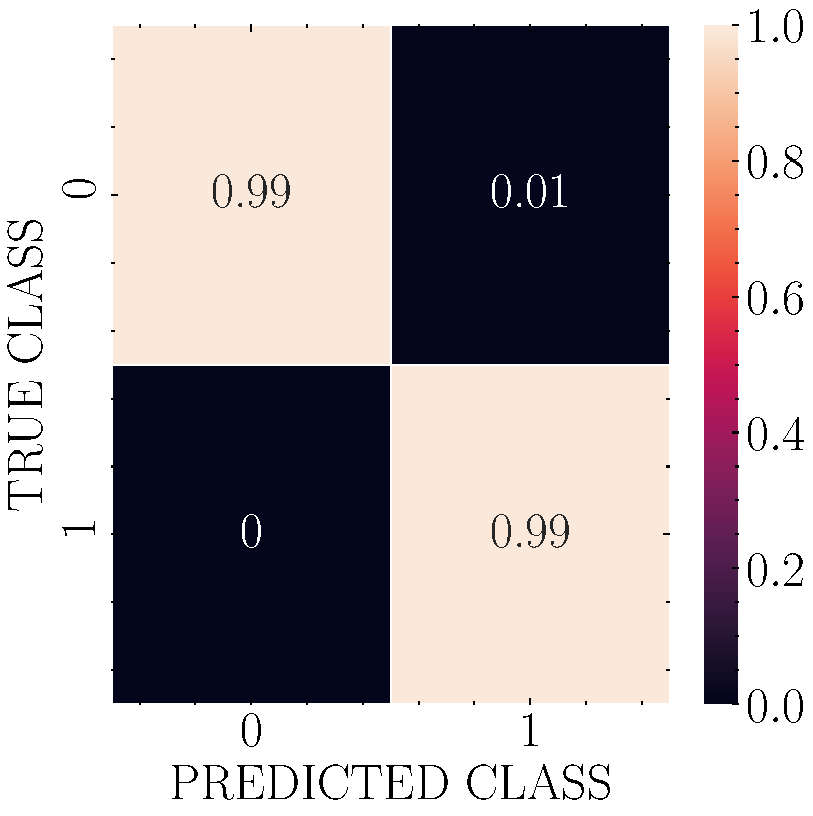
\includegraphics[width=1.8in]{../results/ex1/conf_mtx_QD_ML_dataset_P1c_size_25.pdf}
       \caption{QDA, size $25$.}
       \label{fig:KNN_P1c_25}
    \end{subfigure}
\quad \quad
    \begin{subfigure}[!htbp]{0.24\textwidth}
       \centering
       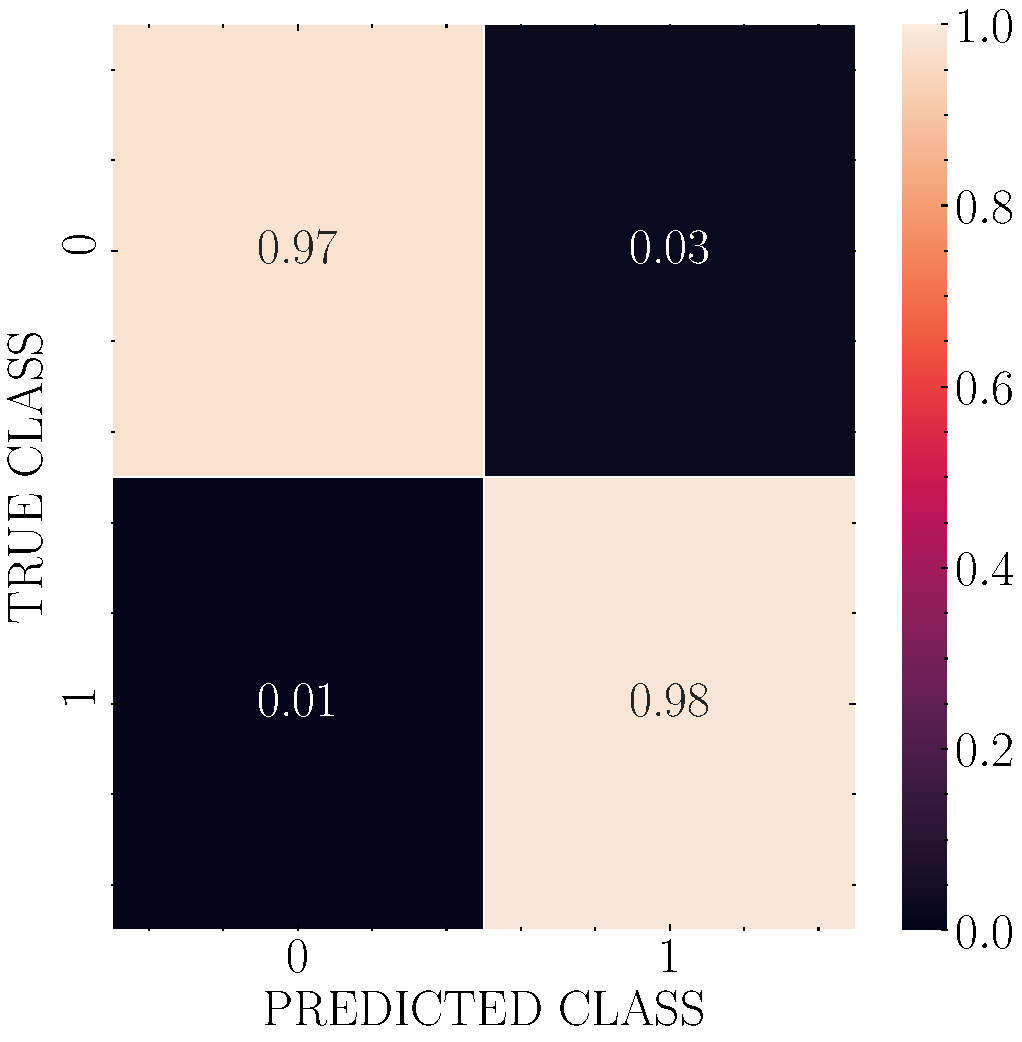
\includegraphics[width=1.8in]{../results/ex1/conf_mtx_KNN_dataset_P1c_size_25.pdf}
       \caption{KNN, size $25$.}
       \label{fig:KNN_P1c_25}
    \end{subfigure}
\quad \quad
    \begin{subfigure}[!htbp]{0.24\textwidth}
       \centering
       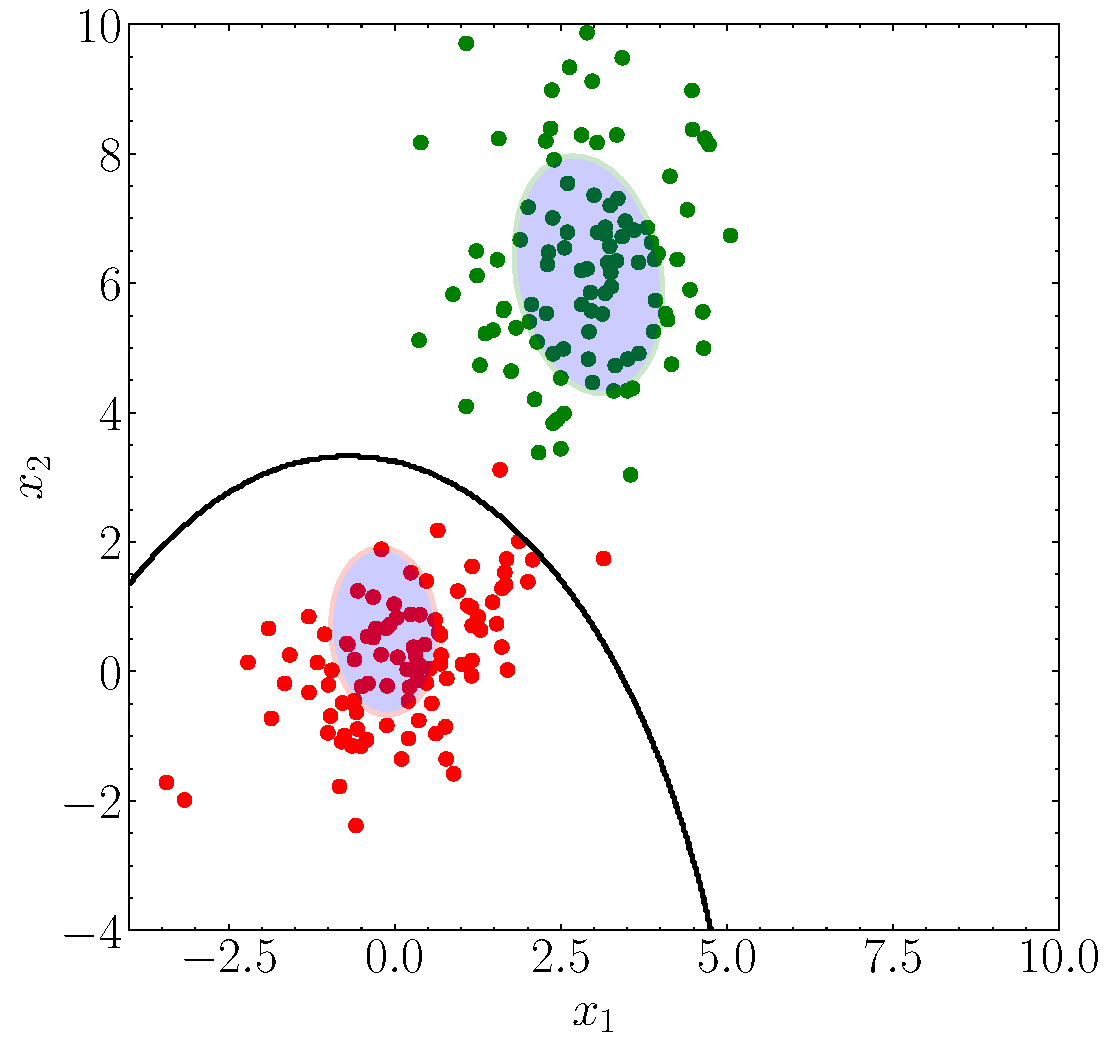
\includegraphics[width=1.8in]{../results/ex1/samples_QD_ML_dataset_P1c_size_25.pdf}
       \caption{Samples, size $25$.}
       \label{fig:KNN_P1c_25}
    \end{subfigure}
    
\quad \quad 
    \begin{subfigure}[!htbp]{0.24\textwidth}
       \centering
       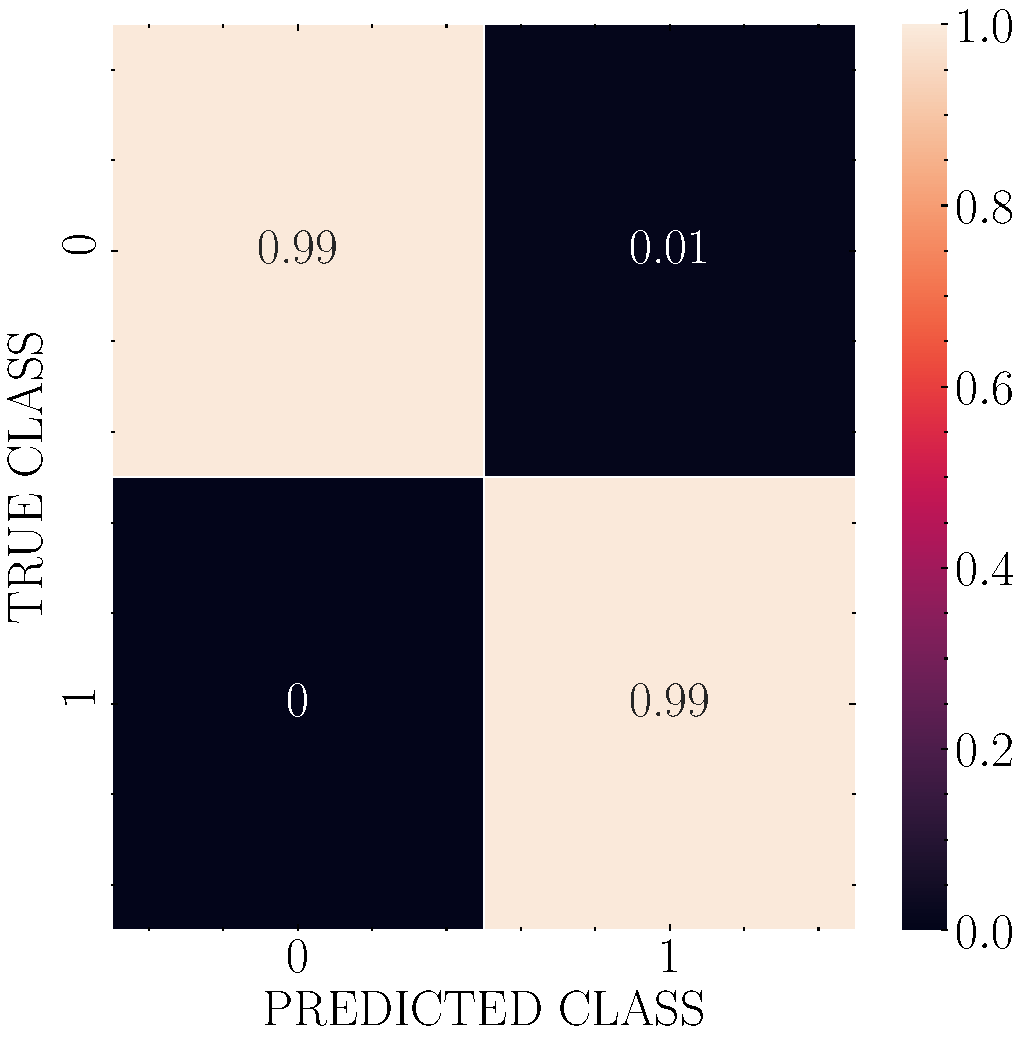
\includegraphics[width=1.8in]{../results/ex1/conf_mtx_QD_ML_dataset_P1c_size_75.pdf}
       \caption{QDA, size $75$.}
       \label{fig:KNN_P1c_75}
    \end{subfigure}
\quad \quad
    \begin{subfigure}[!htbp]{0.24\textwidth}
       \centering
       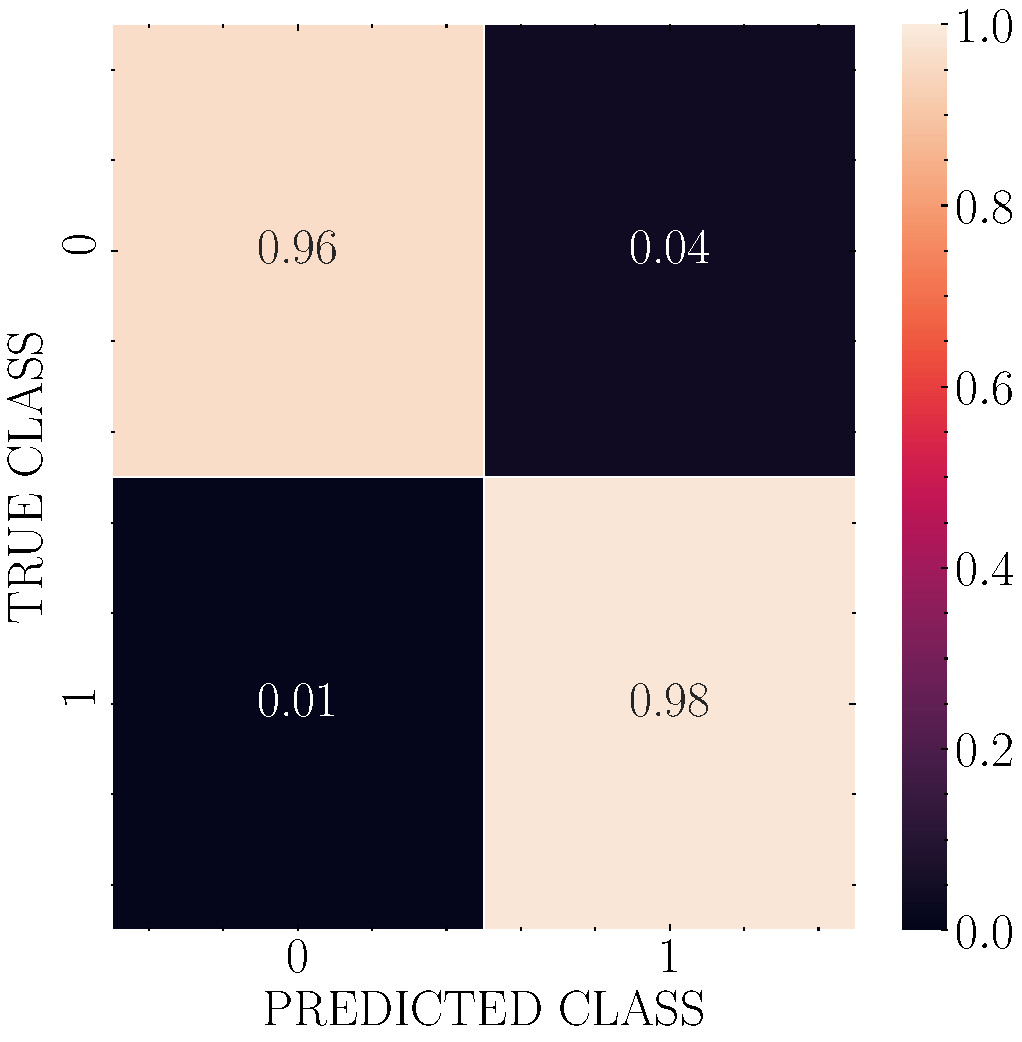
\includegraphics[width=1.8in]{../results/ex1/conf_mtx_KNN_dataset_P1c_size_75.pdf}
       \caption{KNN, size $75$.}
       \label{fig:KNN_P1c_75}
    \end{subfigure}
\quad \quad
    \begin{subfigure}[!htbp]{0.24\textwidth}
       \centering
       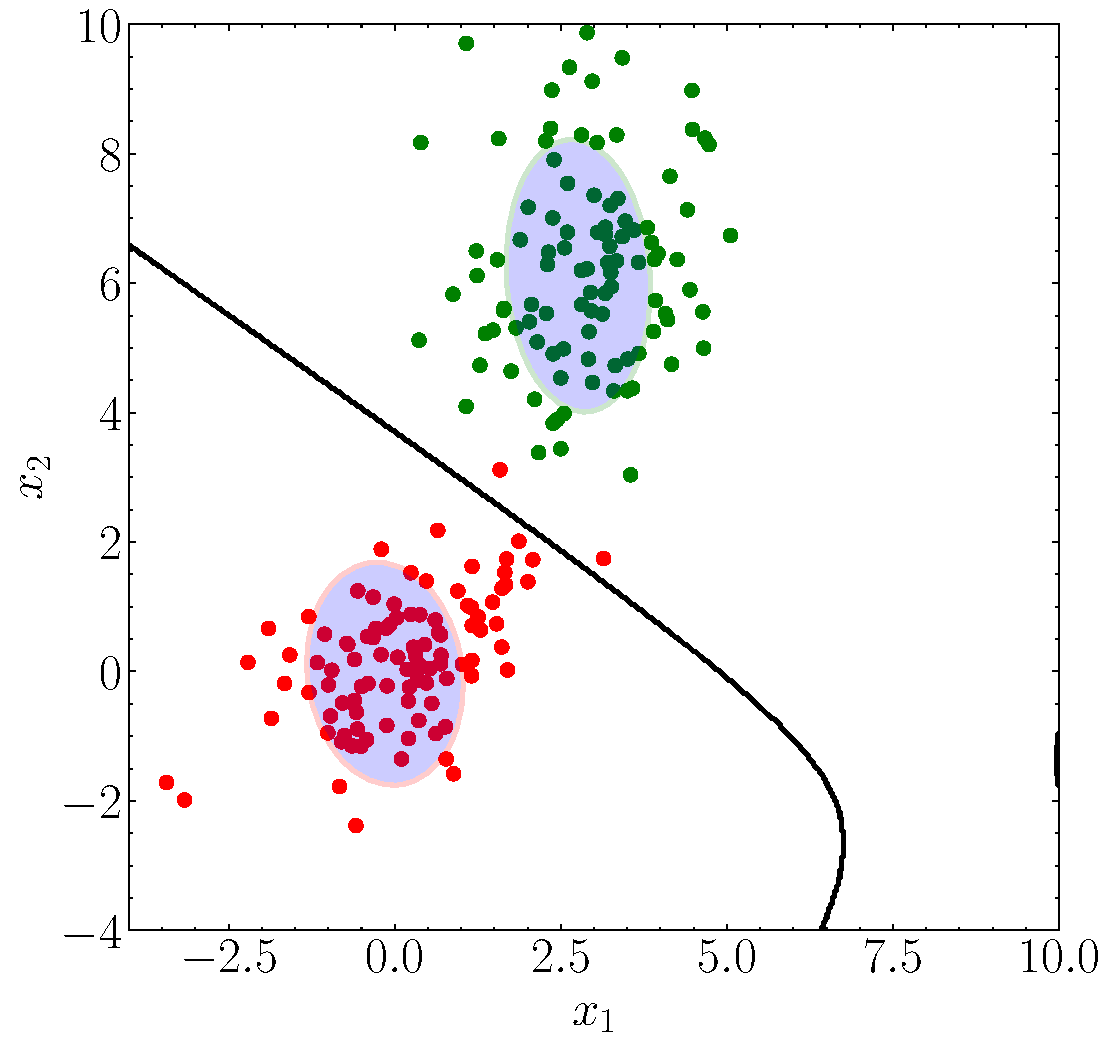
\includegraphics[width=1.8in]{../results/ex1/samples_QD_ML_dataset_P1c_size_75.pdf}
       \caption{Samples, size $75$.}
       \label{fig:KNN_P1c_75}
    \end{subfigure}
    
\quad \quad
    \begin{subfigure}[!htbp]{0.24\textwidth}
       \centering
       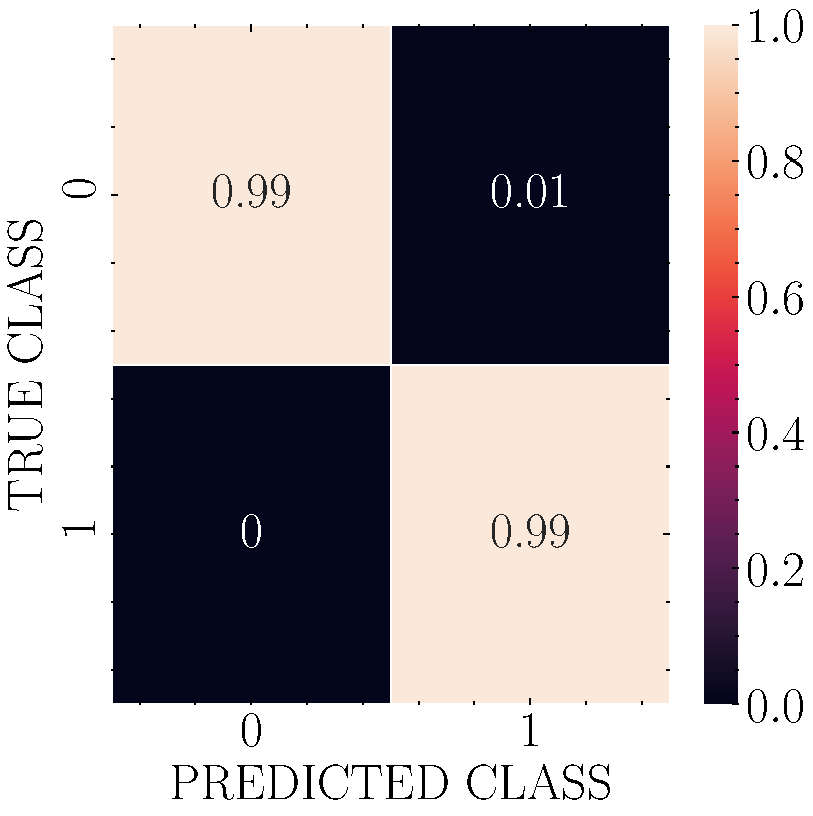
\includegraphics[width=1.8in]{../results/ex1/conf_mtx_QD_ML_dataset_P1c_size_199.pdf}
       \caption{QDA, size $199$.}
       \label{fig:KNN_P1c_199}
    \end{subfigure}
\quad \quad
    \begin{subfigure}[!htbp]{0.24\textwidth}
       \centering
       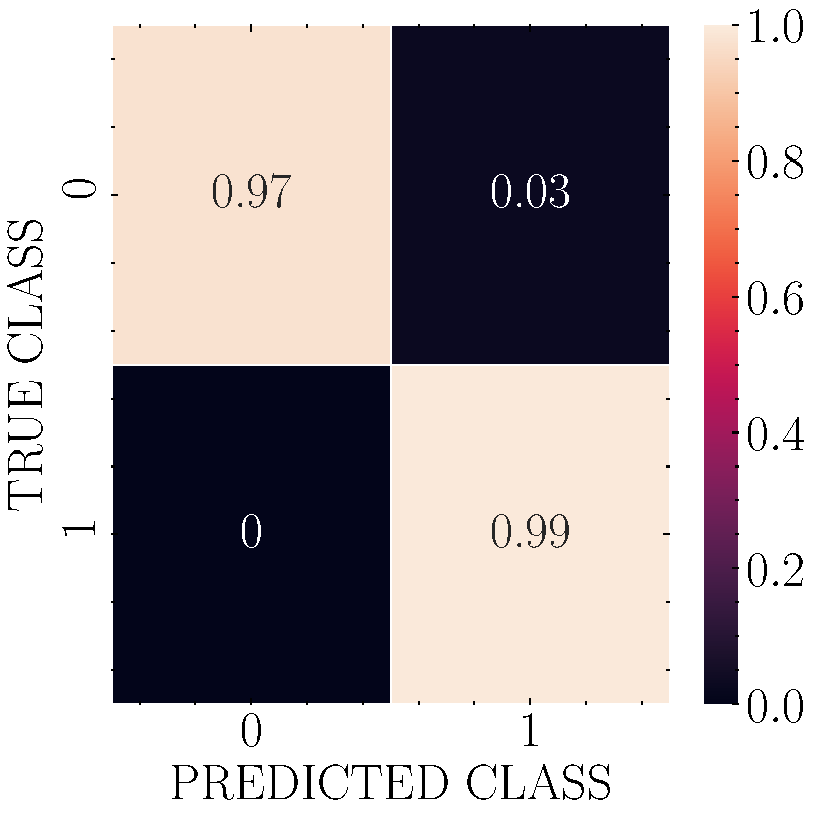
\includegraphics[width=1.8in]{../results/ex1/conf_mtx_KNN_dataset_P1c_size_199.pdf}
       \caption{KNN, size $199$.}
       \label{fig:KNN_P1c_199}
    \end{subfigure}
\quad \quad
    \begin{subfigure}[!htbp]{0.24\textwidth}
       \centering
       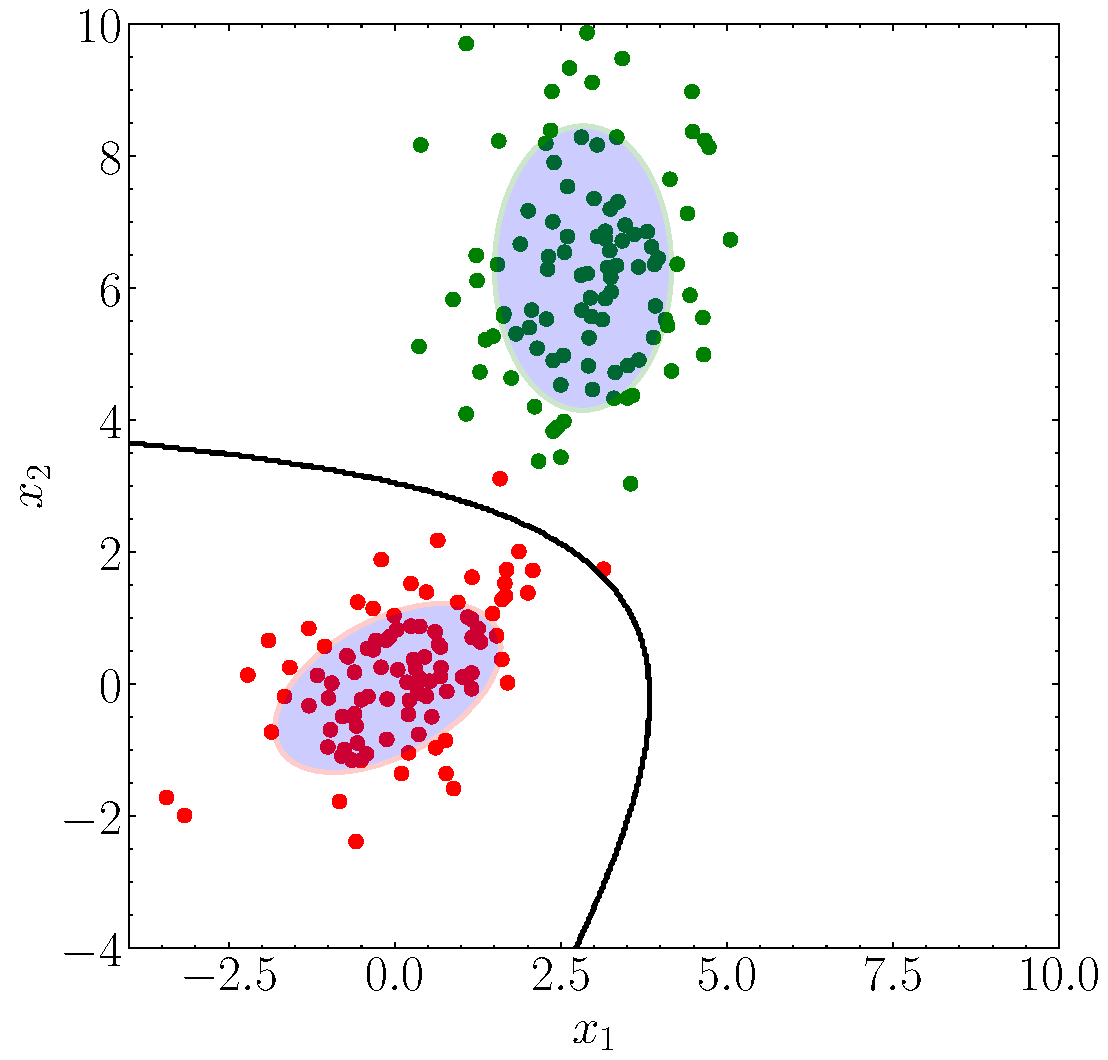
\includegraphics[width=1.8in]{../results/ex1/samples_QD_ML_dataset_P1c_size_199.pdf}
       \caption{Samples, size $199$.}
       \label{fig:KNN_P1c_199}
    \end{subfigure}
\caption{Bayes classifier and Nearest neighbour classification on P1c dataset.}
\label{fig:ex11P1c}
\end{figure}
\underline {\it \bfseries Inferences on P1c}: The class means are $\bmu_{0} = [0 \; 0]^{\TT}$ and $\bmu_{1} = [3 \; 6]^{\TT}$, and the covariances are in the same order. The class distributions are far apart, i.e., the discriminability is high. This is seen with the training samples from each class not overlapping into the other class. Within this setting, the classifiers trained with training sizes $10$, $25$, $75$, and $199$ on the average show, show an increasing trend in test accuracy. In the case where all the training samples are used, the accuracy in classification on the test data is $99\%$. When the data distributions are well separated, risk minimisation is achieved with training sample size as small as $199$ pairs. The nearest-neighbour classifier performs comparably to the Bayes' classifier. In most cases, the error in classification using nearest-neighbour classifier does not exceed twice the error in the Bayes' classifier. With increasing size of the training set, the learnt Gaussians is observed to learn ``better'', i.e., the means and covariances are closer to the true values. \\

% ------------------------------------------------------------------------------------------------------------------------------------------------------

\problem{Problem (1.2) Bayes' Classifier Trained using Gaussian Mixture Model}
\label{prob:1.2}
Let the distribution of the data be modelled to be a mixture of two Gaussians. Here, the class labels are not important to learn the Gaussian mixtures as both classes are learnt together. The data distribution has the density function:
\begin{equation}
	f(\bx; \btheta) = \sum_{i=0}^{1} \lambda_{i} f_{i}(\bx; \bmu_{i}, \bSigma_{i}),
\label{eq:gmmModel}
\end{equation}
where $f_{i}$ are Gaussians as in (\ref{eq:mvGaussian}) and $\btheta = [\lambda_{0} \; \lambda_{1} \; \bmu_{0} \; \bmu_{1} \; \bSigma_{0} \; \bSigma_{1}]$ is the vector of unknowns to be estimated during the training phase using the training samples. \\

\underline {\it \bfseries Implementation}: The maximum likelihood estimation (MLE) is performed using the expectation maximisation (EM) algorithm. The E-step updates the weight matrix:
\begin{equation}
	\gamma_{i,j}^{(k+1)} = \frac{\lambda_{j}^{(k+1)} f_{i}(\bx^{(i)}; \bmu_{j}^{(k+1)}, \bSigma_{j}^{{(k+1)}})}{\sum_{m=0}^{1} \lambda_{m}^{(k+1)} f_{i}(\bx^{(i)}; \bmu_{m}^{(k+1)}, \bSigma_{m}^{(k+1)})},
\label{eq:estep}
\end{equation}
where the $(k+1)$st update for the priors, means and covariances are obtained in the M-step with:
\begin{equation}
\begin{split}
	\bmu_{j}^{(k+1)} &= \frac{\sum_{i=1}^{n} \gamma^{(k)}_{i,j} \bx^{(i)}}{\sum_{i=1}^{n} \gamma^{(k)}_{i,j}}, \\
	\lambda_{j}^{(k+1)} &= \frac{1}{n} \sum_{i=1}^{n} \gamma^{(k)}_{i,j}, \\
	\bSigma_{j}^{(k+1)} &= \frac{\sum_{i=1}^{n} \gamma^{(k)}_{i,j} (\bx^{(i)} - \bmu_{j}^{(k)})(\bx^{(i)} - \bmu_{j}^{(k)})^{\TT}}{\sum_{i=1}^{n} \gamma^{(k)}_{i,j}}.
\end{split}
\label{eq:mstep}
\end{equation}
Each component in Gaussian mixture is considered to be the class conditional and the corresponding Bayes' classifier in (\ref{eq:bayesClassifier}) is tested on the test dataset. The classifier is trained on the P1b dataset using all training samples. The trained classifier is tested in the full test dataset and the confusion matrix and the discriminant functions are plotted. The classifier is compared with the class conditional modelled as Gaussians as in Problem \ref{prob:1.1}.1. \\

\underline {\it \bfseries Results}: Figure \ref{fig:ex12P1b} shows the results for testing the classifier on P1b dataset. Figure \ref{fig:gmmLoss} shows the log-likelihood function $\ell(\btheta) = \ln f(\bx; \btheta)$ for the parameter vector $\btheta$. Figures \ref{fig:GMM_P1b} and \ref{fig:GMM_QDA_P1b} shows the accuracies in the confusion matrix for the classifier trained with GMM and individual Gaussian classes, respectively. Figures \ref{fig:GMM_DF_P1b} and \ref{fig:QDA_DF_P1b} show the training samples (red samples in class 0, green samples in class 1), the $3-\sigma$ Gaussian learnt from the training samples (ellipses of the corresponding colours), and the quadratic discriminant function (black).

\begin{figure}[!htbp]
\centering
\quad
    \begin{subfigure}[!htbp]{0.24\textwidth}
       \centering
       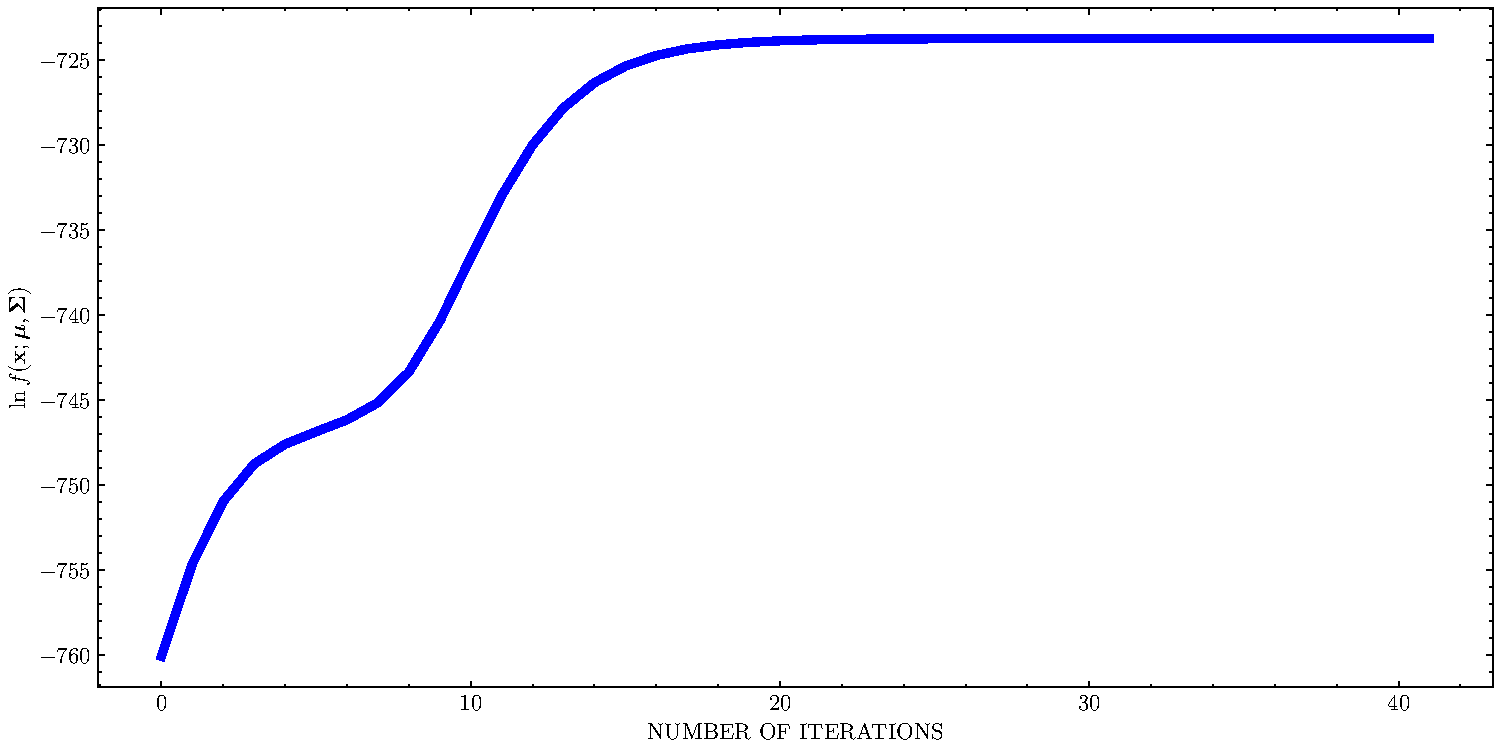
\includegraphics[width=1.8in]{../results/ex1/loss_GMM_EM_dataset_P1b_size_199.pdf}
       \caption{$\ell(\btheta)$.}
       \label{fig:gmmLoss}
    \end{subfigure}
\quad \quad
    \begin{subfigure}[!htbp]{0.24\textwidth}
       \centering
       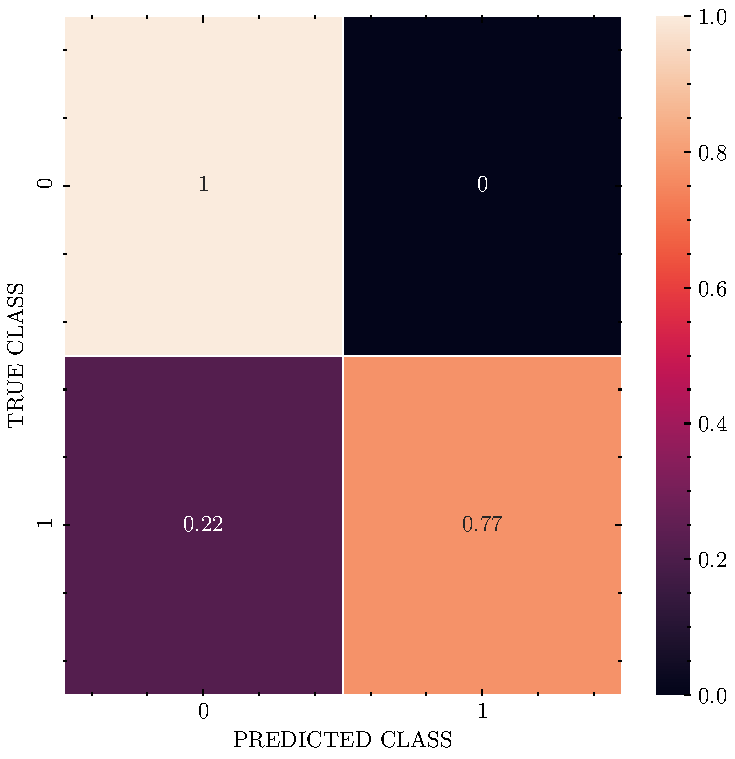
\includegraphics[width=1.8in]{../results/ex1/conf_mtx_GMM_EM_dataset_P1b_size_199.pdf}
       \caption{GMM.}
       \label{fig:GMM_P1b}
    \end{subfigure}
\quad \quad
    \begin{subfigure}[!htbp]{0.24\textwidth}
       \centering
       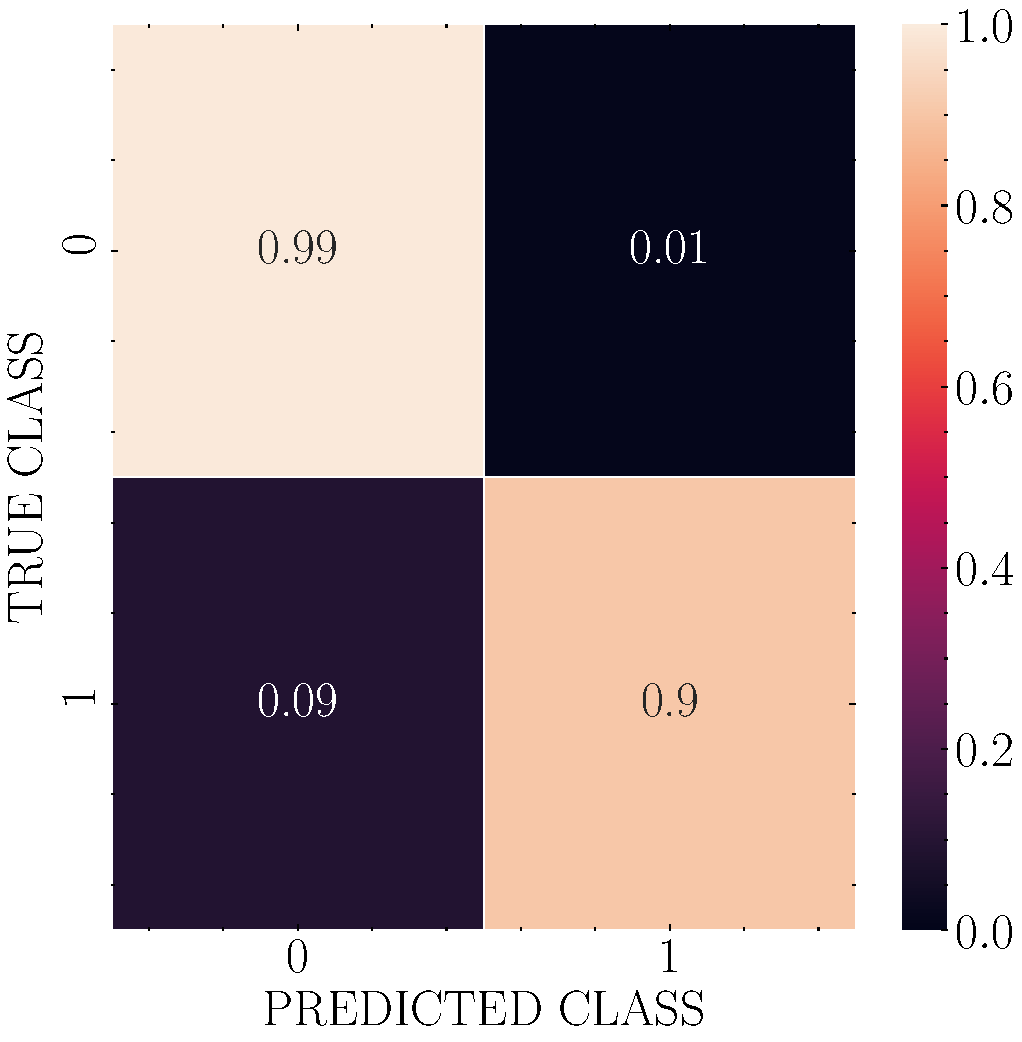
\includegraphics[width=1.8in]{../results/ex1/conf_mtx_QD_ML_dataset_P1b_size_199.pdf}
       \caption{QDA.}
       \label{fig:GMM_QDA_P1b}
    \end{subfigure}
\\
    \begin{subfigure}[!htbp]{0.24\textwidth}
       \centering
       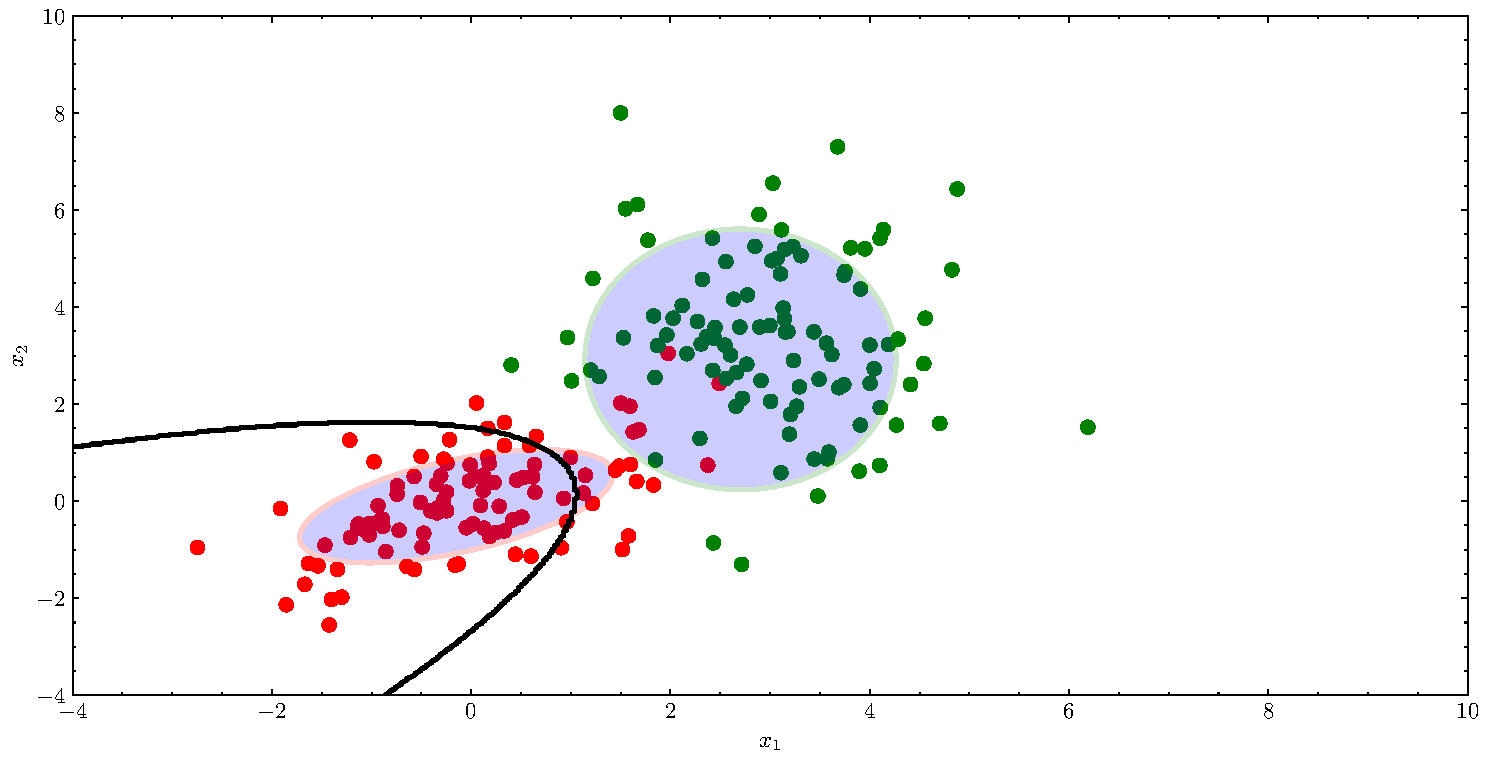
\includegraphics[width=1.8in]{../results/ex1/samples_GMM_EM_dataset_P1b_size_199.pdf}
       \caption{Samples, GMM.}
       \label{fig:GMM_DF_P1b}
    \end{subfigure}
\quad \quad
    \begin{subfigure}[!htbp]{0.24\textwidth}
       \centering
       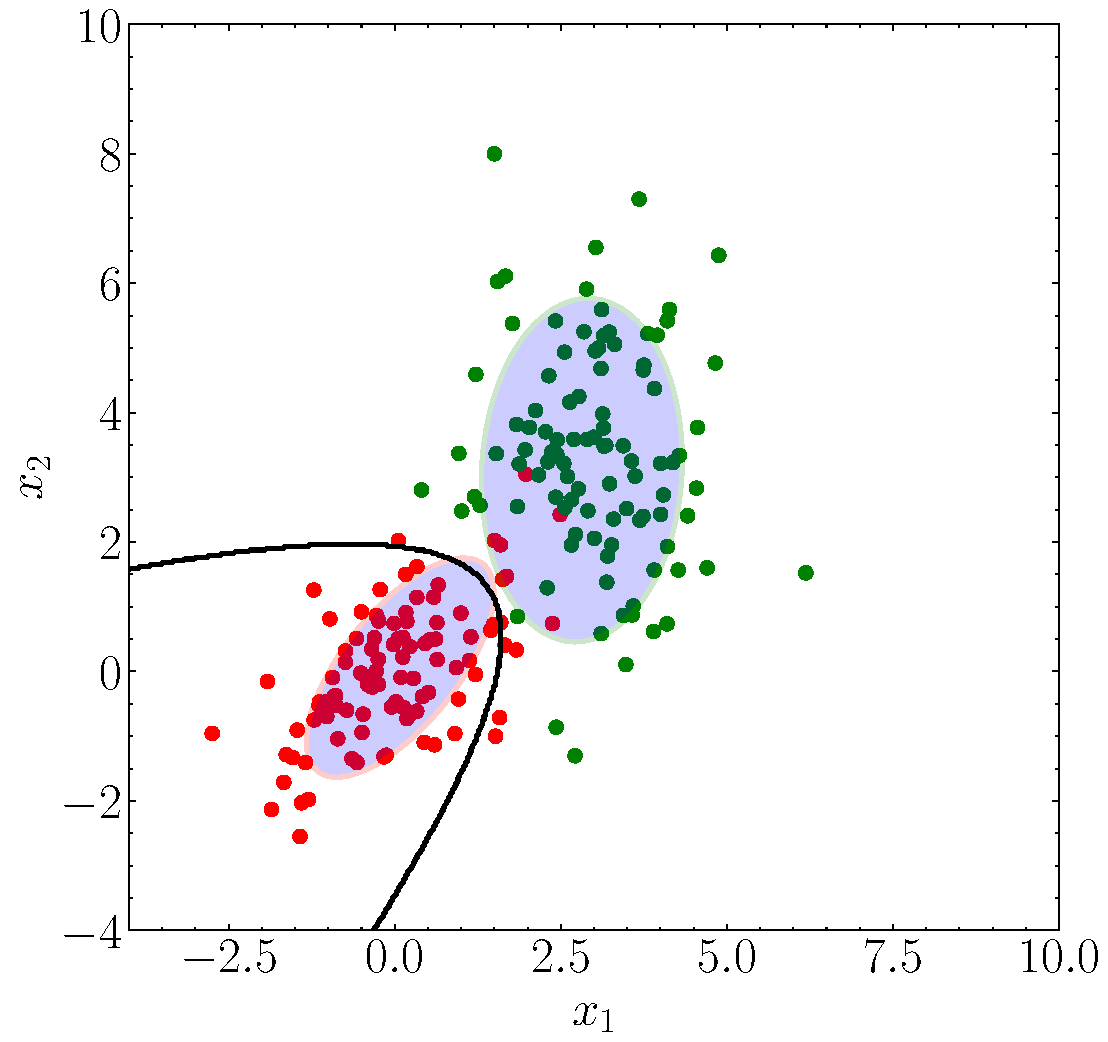
\includegraphics[width=1.8in]{../results/ex1/samples_QD_ML_dataset_P1b_size_199.pdf}
       \caption{Samples, QDA.}
       \label{fig:QDA_DF_P1b}
    \end{subfigure}
\caption{Bayes classifier learnt using Gaussian mixture model and each class modelled as Gaussian on P1b dataset.}
\label{fig:ex12P1b}
\end{figure}
\underline {\it \bfseries Inferences}: Figure \ref{fig:gmmLoss} shows the log-likelihood function for $\btheta$ and it can be observed that the EM algorithm maximises the log-likelihood and convergence is achieved in $34$ iterations. Since the entire data distribution is learnt together using GMM, the learning is unsupervised; whereas modelling each class as a Gaussian requires the class labels and is hence supervised. However, the knowledge of the number of components is necessary for training using GMM. The accuracies on the test data using GMM are comparable to the accuracies on the test data using supervised training, and the discriminant functions obtained are also similar.

% ------------------------------------------------------------------------------------------------------------------------------------------------------

\problem{Problem (1.3) Bayes' Classifier with Exponential Class Conditional}
\label{prob:1.3}
Let the class $0$ be modelled as a Gaussian, identical to Problem \ref{prob:1.1}.1 and class $1$ be modelled as independent Exponentials, i.e.:
\begin{equation}
	f_{1}(\bx; \lambda_{1}, \lambda_{2}) = \lambda_{1}\lambda_{2} e^{-\lambda_{1}x_{1} -\lambda_{2}x_{2}},
\label{eq:expConditionalModel}
\end{equation}
where the parameters $\lambda_{1}, \lambda_{2}$ are unknowns that are estimated in the training phase using the training data. \\

\underline{\it \bfseries Implementation}: The maximum-likelihood estimate for the parameters is given by:
\begin{equation}
	\lambda_{j} = \frac{n}{\sum_{i=1}^{n} x_{j}^{(i)}}, \; j=1,2,
\label{eq:mleExp}
\end{equation}
where $n$ is the number of samples in the class. The priors are computed similar to \ref{prob:1.1}.1, as ratios of number of samples in the class to total number of samples. The classifier is trained on the P1c dataset using all the training samples. The trained classifier is tested on the full dataset and the confusion matrix are plotted. The classifier is compared with both class conditionals modelled as Gaussians as in \ref{prob:1.1}.1. \\

\underline{\it \bfseries Results}: Figure \ref{fig:ex13P1c} shows the results for testing the classifier on P1c dataset. Figure \ref{fig:EXP_P1c} shows the accuracies in the confusion matrix for the classifier with Gaussian and Exponential class distributions. Figure \ref{fig:QDA_EXP_P1c} shows the accuracies in the confusion matrix for the classifier with both classes modelled as Gaussians. Figure \ref{fig:samples_P1c} shows the training samples along with the learnt Gaussian for class $0$. \\

\begin{figure}[!htbp]
\centering
    \begin{subfigure}[!htbp]{0.24\textwidth}
       \centering
       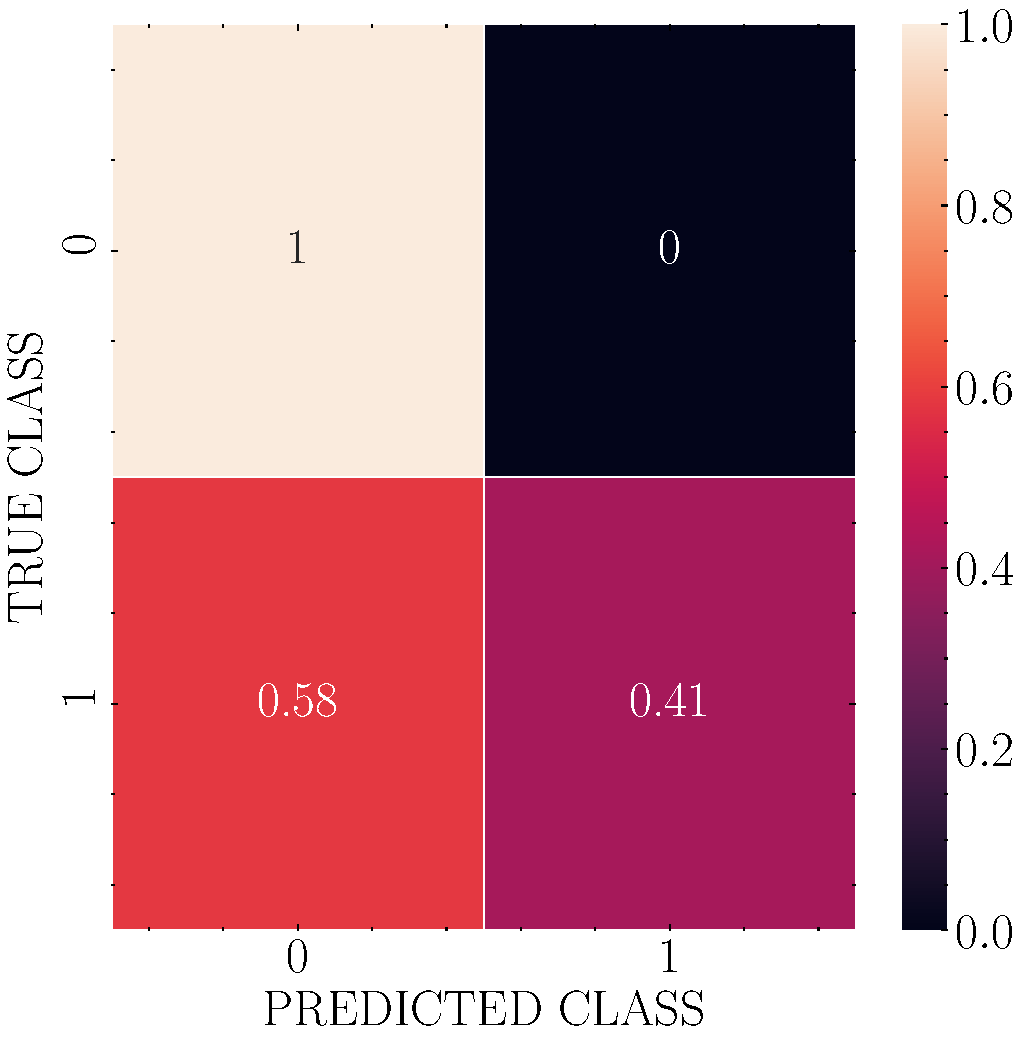
\includegraphics[width=1.8in]{../results/ex1/conf_mtx_QD_EXP_ML_dataset_P1c_size_199.pdf}
       \caption{Exp-Gaussian.}
       \label{fig:EXP_P1c}
    \end{subfigure}
\quad \quad
    \begin{subfigure}[!htbp]{0.24\textwidth}
       \centering
       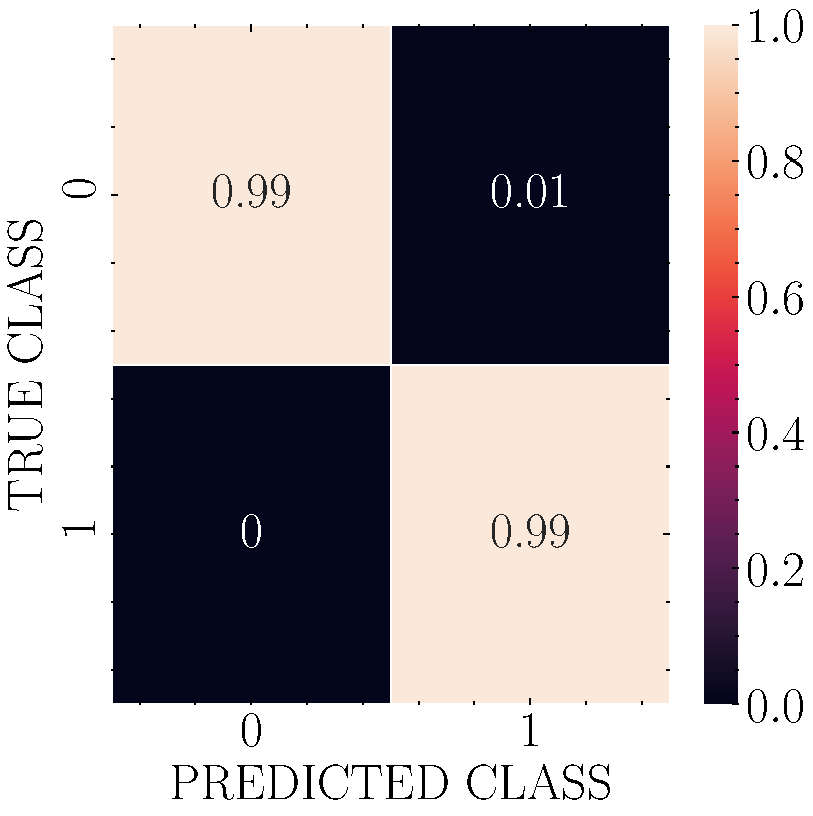
\includegraphics[width=1.8in]{../results/ex1/conf_mtx_QD_ML_dataset_P1c_size_199.pdf}
       \caption{QDA.}
       \label{fig:QDA_EXP_P1c}
    \end{subfigure}
\quad \quad
    \begin{subfigure}[!htbp]{0.24\textwidth}
       \centering
       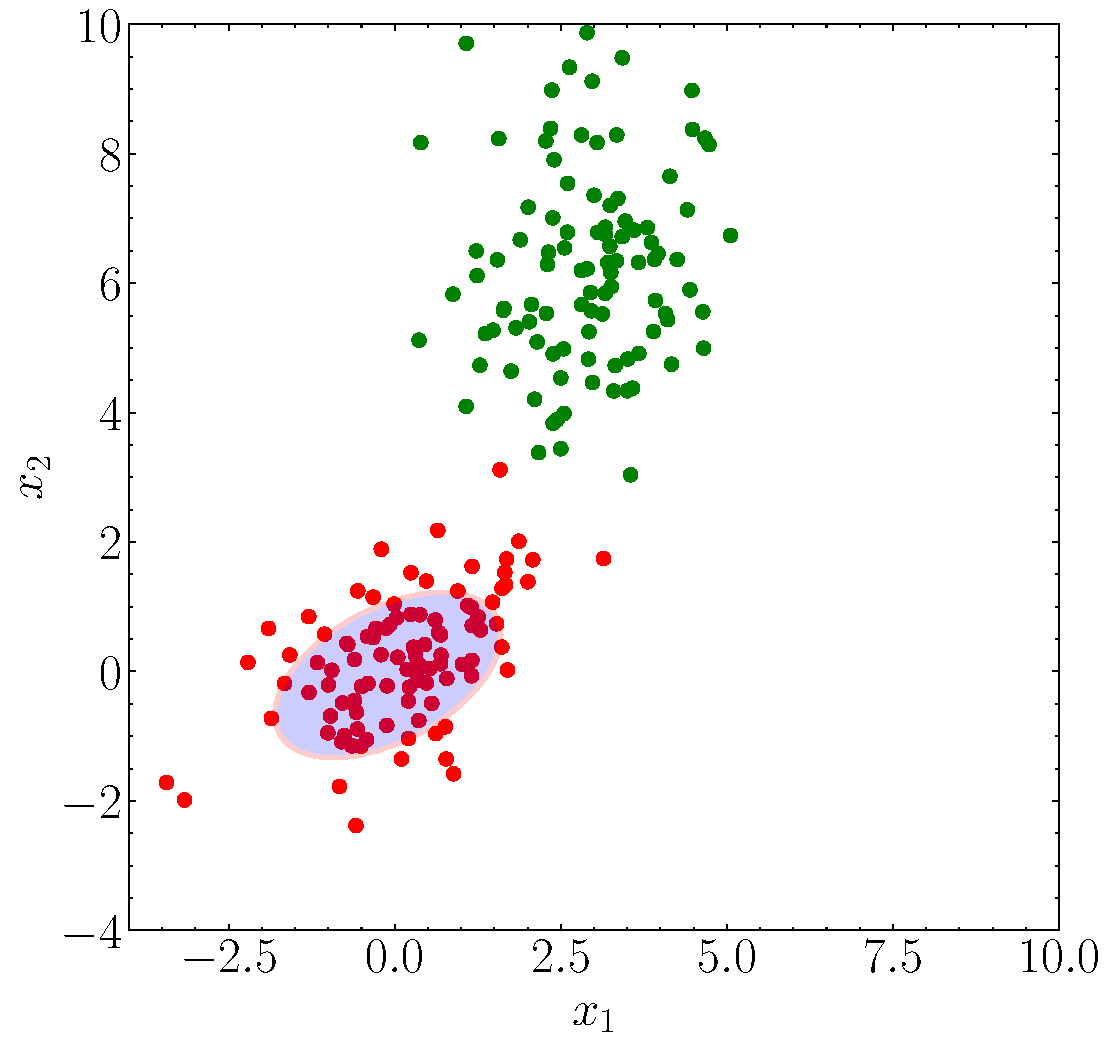
\includegraphics[width=1.8in]{../results/ex1/samples_QD_EXP_ML_dataset_P1c_size_199.pdf}
       \caption{Samples.}
       \label{fig:samples_P1c}
    \end{subfigure}
\caption{Bayes' classifier with class conditionals as Gaussian and Exponential; and both class conditionals as Gaussians on P1c dataset.}
\label{fig:ex13P1c}
\end{figure}
\underline {\it \bfseries Inferences}: The performance of the classifier with exponential distribution is poor. The accuracy of classification into class $0$ with Gaussian class conditional is $100\%$ in comparison to the accuracy of classification with both class conditionals as Gaussians and with GMM. However, the accuracy of classification with the exponential distribution is very poor and comparable to a coin-toss classifier. This is expected as the mean of class $1$ is at $[3\; 6]^{\TT}$ and since the class is exponential, the samples are not drawn from a bell-shape. The samples are drawn around $[0\; 0]^{\TT}$ with high probability. \\

The exponential distribution is not a good model for the class conditional, in this case. This is apparent as we know a priori, the class conditionals are Gaussian. Model mismatch in the modelling of the class conditional explains the poor performance of the classifiers.

% ------------------------------------------------------------------------------------------------------------------------------------------------------
% ------------------------------------------------------------------------------------------------------------------------------------------------------

\section{Bayes' Classifier in $\rr^{20}$}
\label{sec:bayes20D}

\problem{Problem (2) Bayes' Classifier with Gaussian Class Conditionals}
\label{prob:2}
Let the class conditional distributions be modelled to be multivariate Gaussians. In the training phase, the unknown means and covariances of the Gaussians are estimated from the training data. \\

\underline {\it \bfseries Implementation}: The model is identical to the setting in Problem \ref{prob:1.1}.1 and the updates for the unknown means and covariances are identical to (\ref{eq:mleGaussian}). The classifiers are trained on three datasets (P2a, P2b, P2c) with varying training sizes. The trained classifiers are tested on the full test dataset and the accuracies in confusion matrices are plotted. The classifier is compared with the nearest-neighbour classifier. \\

\underline {\it \bfseries Results}: Figure \ref{fig:ex2P2a} shows the results for testing the classifier on P2a dataset. Figure \ref{fig:QDA_rr20_P2a_50} \ref{fig:QDA_rr20_P2a_100} \ref{fig:QDA_rr20_P2a_300} \ref{fig:QDA_rr20_P2a_999} depicts the accuracies in confusion matrices for the Bayes' classifier, Figures \ref{fig:KNN_rr20_P2a_50} \ref{fig:KNN_rr20_P2a_100} \ref{fig:KNN_rr20_P2a_300} \ref{fig:KNN_rr20_P2a_999} depicts the accuracies in confusion matrices for the nearest-neighbour classifier. Figures \ref{fig:ex2P2b} and \ref{fig:ex2P2c} shows the corresponding results for datasets P2b and P2c, respectively. All the datasets have the same means for the classes, $\bmu_{0} = \boldsymbol{0}$ and $\bmu_{1} = \mathbbm{1}$, but different covariances. \\

\underline {\it \bfseries Inferences on P2a}: The covariance matrices of the classes are both equal to the identity matrix. Hence, the discriminability in the data is sufficient and the classifier performs well with sufficient training samples. $10$ samples are insufficient to completely capture the model and the Bayes' classifier performs poorly. The estimated means are not accurate and hence the class conditionals are not accurate. The nearest-neighbour classifier performs well with $10$ samples. With few training samples, the nearest-neighbour classifier is more reliable than the Bayes' classifier. As the number of training samples increase from $10$ to $50$, $100$ and $300$, the performance of the Bayes' classifier beats nearest-neighbour, as in these cases, the MLE converges to the true values. The error in nearest-neighbour classification is at most twice the error in Bayes' classifier, in most cases. \\

\underline {\it \bfseries Inferences on P2b}: The covariance matrices of the classes are both equal to three times the identity matrix. Hence, the discriminability in the data is insufficient. The data from either of the classes overlap into the other class. The classifiers perform poorly in relation to P2a, where the discriminability is better. The number of samples taken in the range of $50$-$100$ are not sufficient of risk minimisation for the data with overlapping classes. In this range of training samples, the nearest neighbour classifier performs better than the Bayes' classifier. As the number of training samples increases to the full training data size, the estimation accuracy improves and the accuracy of the classifier improves. Again, when the estimation of the parameters improves, the error in the nearest-neighbour classifier is less than twice the error in Bayes' classifier. \\
\begin{figure}[!htbp]
\centering
    \begin{subfigure}[!htbp]{0.24\textwidth}
       \centering
       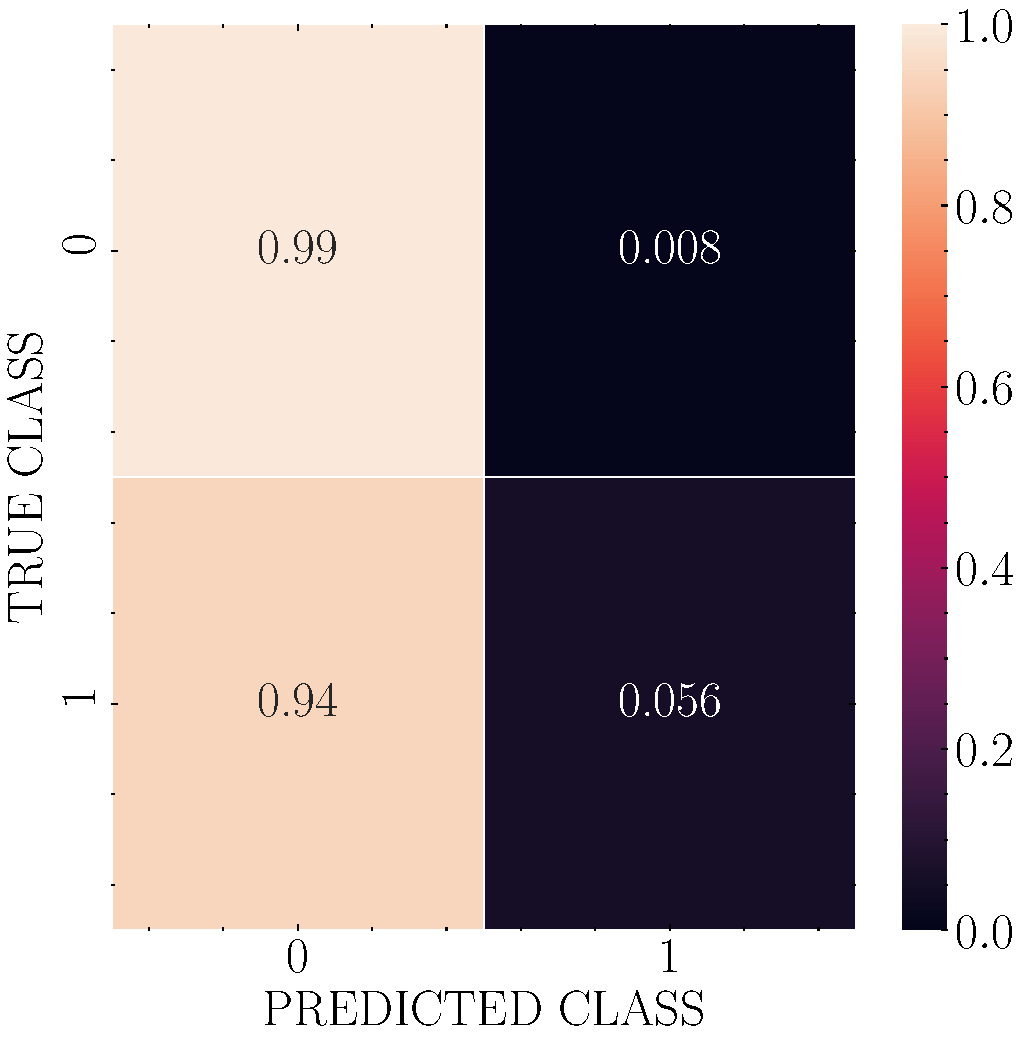
\includegraphics[width=1.8in]{../results/ex2/conf_mtx_QD_ML_dataset_P2a_size_50.pdf}
       \caption{QDA, size $50$.}
       \label{fig:QDA_rr20_P2a_50}
    \end{subfigure}
\quad \quad
    \begin{subfigure}[!htbp]{0.24\textwidth}
       \centering
       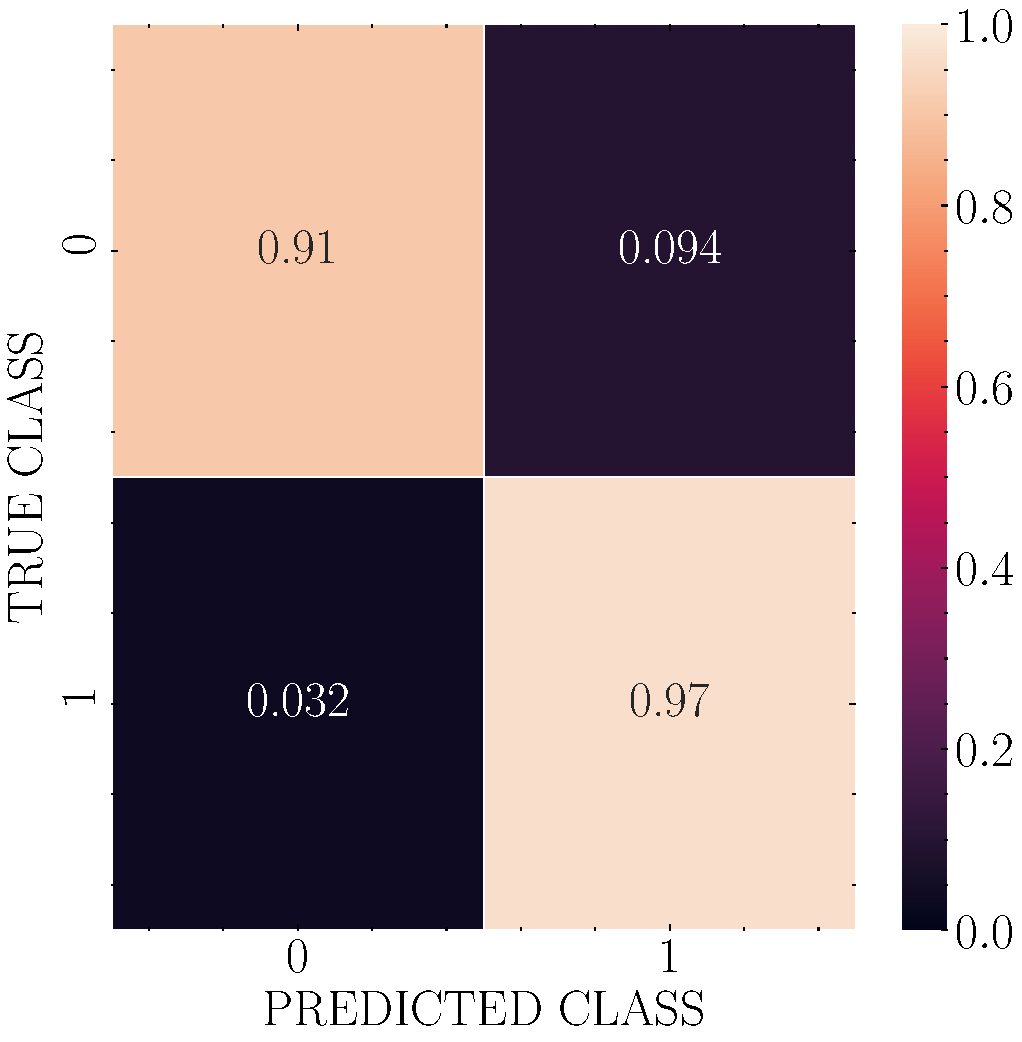
\includegraphics[width=1.8in]{../results/ex2/conf_mtx_KNN_dataset_P2a_size_50.pdf}
       \caption{KNN, size $50$.}
       \label{fig:KNN_rr20_P2a_50}
    \end{subfigure}
\\  
    \begin{subfigure}[!htbp]{0.24\textwidth}
       \centering
       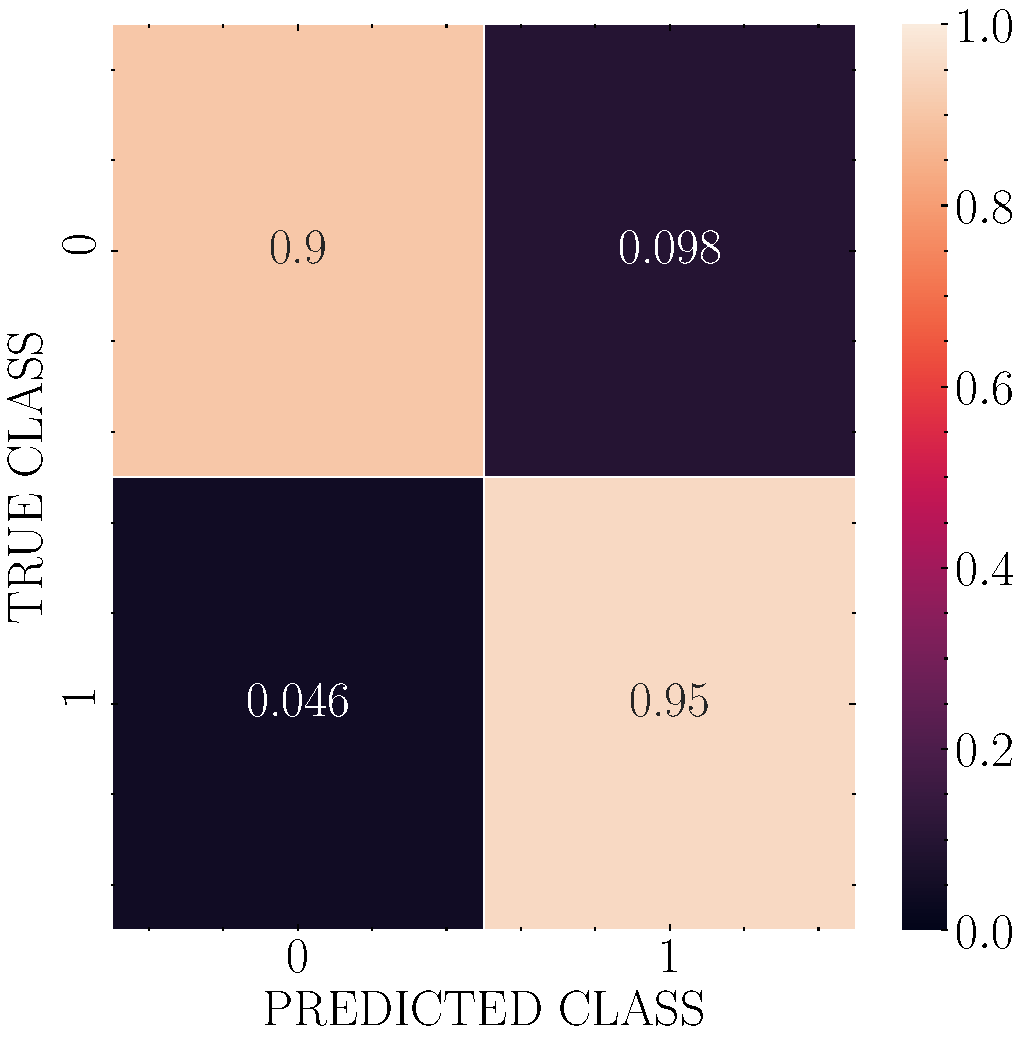
\includegraphics[width=1.8in]{../results/ex2/conf_mtx_QD_ML_dataset_P2a_size_100.pdf}
       \caption{QDA, size $100$.}
       \label{fig:QDA_rr20_P2a_100}
    \end{subfigure}
\quad \quad
    \begin{subfigure}[!htbp]{0.24\textwidth}
       \centering
       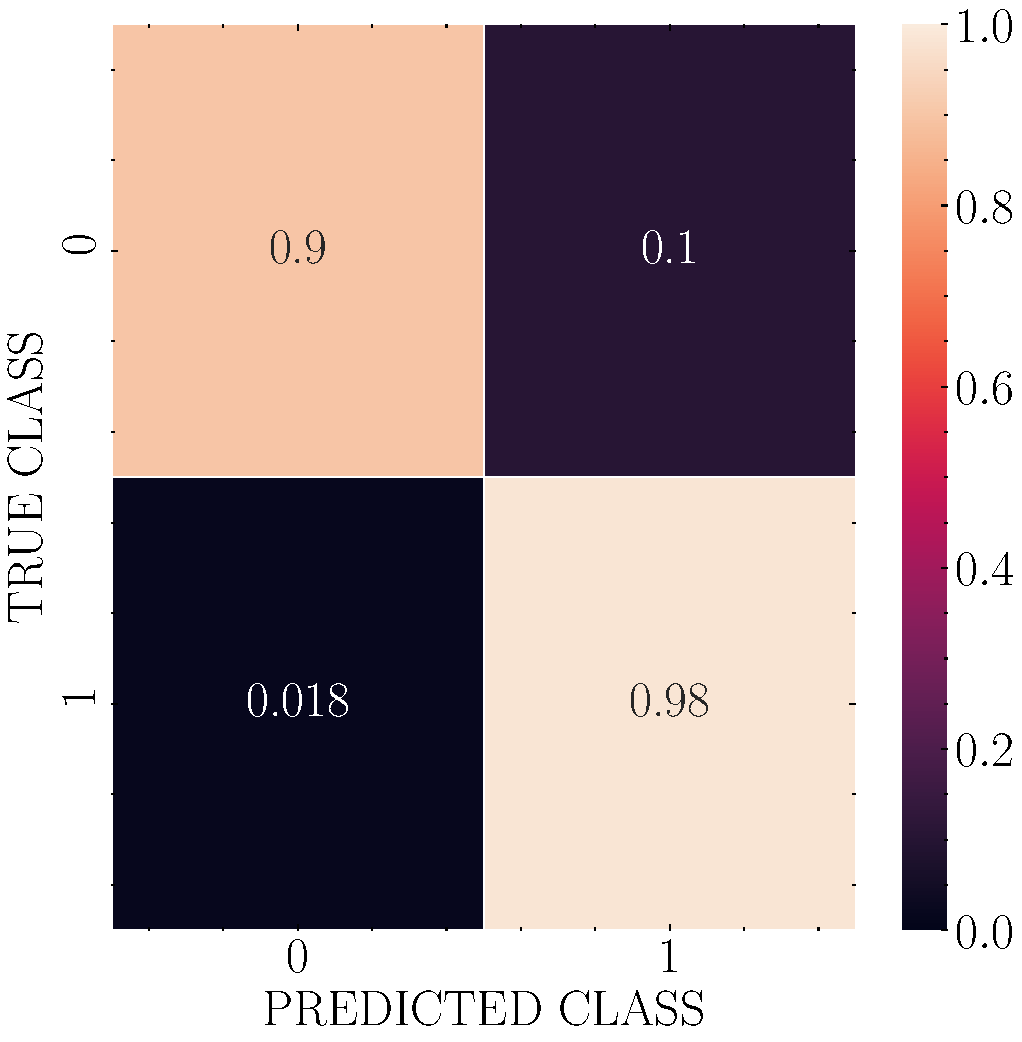
\includegraphics[width=1.8in]{../results/ex2/conf_mtx_KNN_dataset_P2a_size_100.pdf}
       \caption{KNN, size $100$.}
       \label{fig:KNN_rr20_P2a_100}
    \end{subfigure}
\\
    \begin{subfigure}[!htbp]{0.24\textwidth}
       \centering
       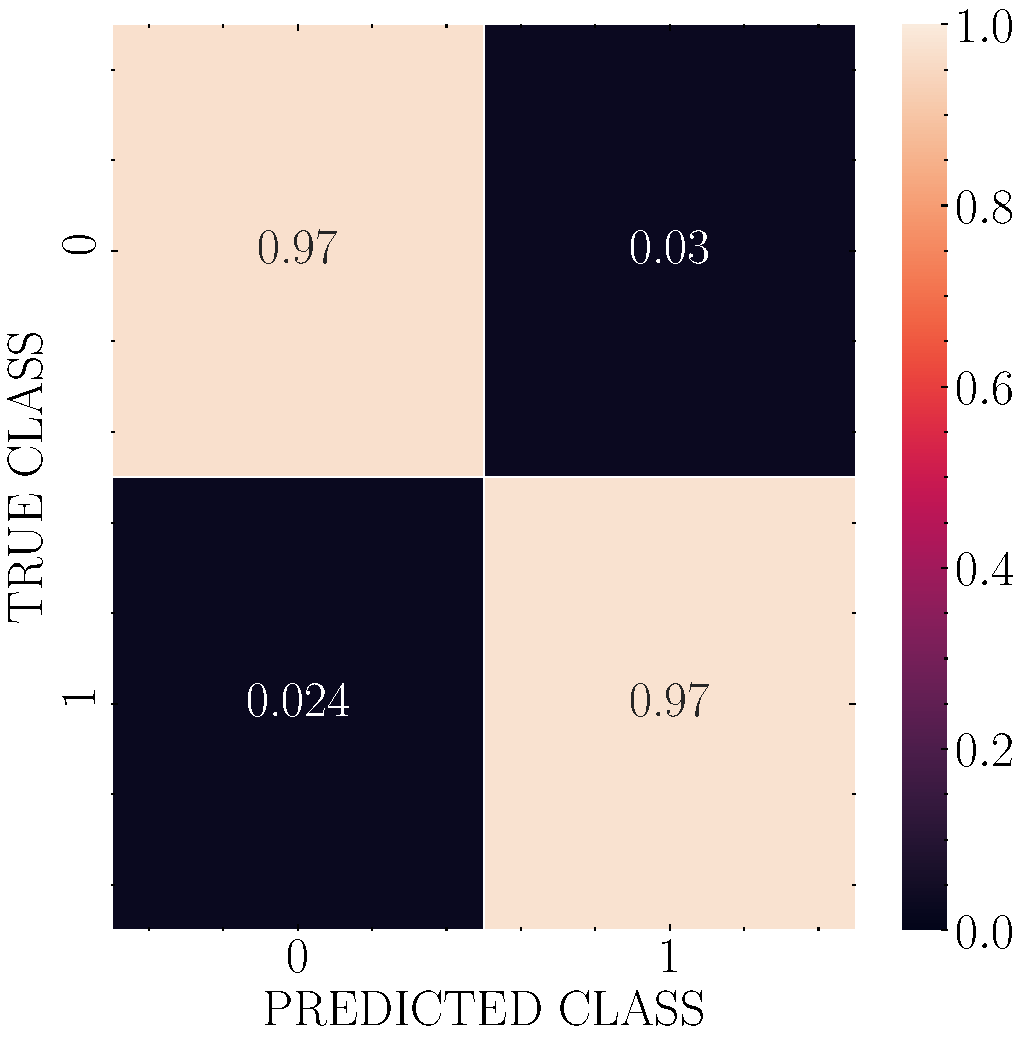
\includegraphics[width=1.8in]{../results/ex2/conf_mtx_QD_ML_dataset_P2a_size_300.pdf}
       \caption{QDA, size $300$.}
       \label{fig:QDA_rr20_P2a_300}
    \end{subfigure}
\quad \quad   
    \begin{subfigure}[!htbp]{0.24\textwidth}
       \centering
       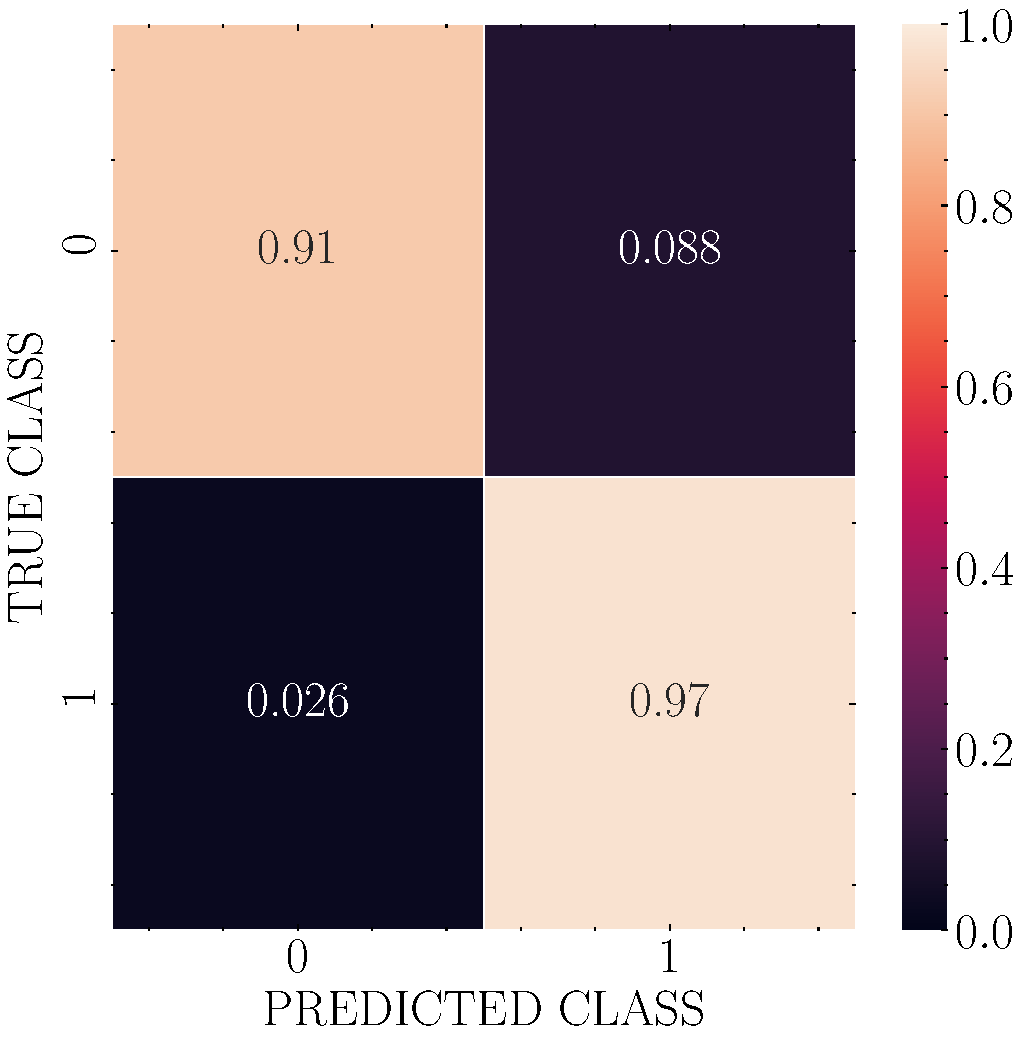
\includegraphics[width=1.8in]{../results/ex2/conf_mtx_KNN_dataset_P2a_size_300.pdf}
       \caption{KNN, size $300$.}
       \label{fig:KNN_rr20_P2a_300}
    \end{subfigure}
\\
    \begin{subfigure}[!htbp]{0.24\textwidth}
       \centering
       \includegraphics[width=1.8in]{../results/ex2/conf_mtx_QD_ML_dataset_P2a_size_999.pdf}
       \caption{QDA, size $999$.}
       \label{fig:QDA_rr20_P2a_999}
    \end{subfigure}
\quad \quad
    \begin{subfigure}[!htbp]{0.24\textwidth}
       \centering
       \includegraphics[width=1.8in]{../results/ex2/conf_mtx_KNN_dataset_P2a_size_999.pdf}
       \caption{KNN, size $999$.}
       \label{fig:KNN_rr20_P2a_999}
    \end{subfigure}
\caption{Bayes classifier and Nearest neighbour classification on P2a dataset.}
\label{fig:ex2P2a}
\end{figure}

\begin{figure}[!htbp]
\centering
    \begin{subfigure}[!htbp]{0.24\textwidth}
       \centering
       \includegraphics[width=1.8in]{../results/ex2/conf_mtx_QD_ML_dataset_P2b_size_50.pdf}
       \caption{QDA, size $50$.}
       \label{fig:QDA_rr20_P2b_50}
    \end{subfigure}
\quad \quad
    \begin{subfigure}[!htbp]{0.24\textwidth}
       \centering
       \includegraphics[width=1.8in]{../results/ex2/conf_mtx_KNN_dataset_P2b_size_50.pdf}
       \caption{KNN, size $50$.}
       \label{fig:KNN_rr20_P2b_50}
    \end{subfigure}
\\  
    \begin{subfigure}[!htbp]{0.24\textwidth}
       \centering
       \includegraphics[width=1.8in]{../results/ex2/conf_mtx_QD_ML_dataset_P2b_size_100.pdf}
       \caption{QDA, size $100$.}
       \label{fig:QDA_rr20_P2b_100}
    \end{subfigure}
\quad \quad
    \begin{subfigure}[!htbp]{0.24\textwidth}
       \centering
       \includegraphics[width=1.8in]{../results/ex2/conf_mtx_KNN_dataset_P2b_size_100.pdf}
       \caption{KNN, size $100$.}
       \label{fig:KNN_rr20_P2b_100}
    \end{subfigure}
\\
    \begin{subfigure}[!htbp]{0.24\textwidth}
       \centering
       \includegraphics[width=1.8in]{../results/ex2/conf_mtx_QD_ML_dataset_P2b_size_300.pdf}
       \caption{QDA, size $300$.}
       \label{fig:QDA_rr20_P2b_300}
    \end{subfigure}
\quad \quad
    \begin{subfigure}[!htbp]{0.24\textwidth}
       \centering
       \includegraphics[width=1.8in]{../results/ex2/conf_mtx_KNN_dataset_P2b_size_300.pdf}
       \caption{KNN, size $300$.}
       \label{fig:KNN_rr20_P2b_300}
    \end{subfigure}
\\
    \begin{subfigure}[!htbp]{0.24\textwidth}
       \centering
       \includegraphics[width=1.8in]{../results/ex2/conf_mtx_QD_ML_dataset_P2b_size_999.pdf}
       \caption{QDA, size $999$.}
       \label{fig:QDA_rr20_P2b_999}
    \end{subfigure}
\quad \quad
    \begin{subfigure}[!htbp]{0.24\textwidth}
       \centering
       \includegraphics[width=1.8in]{../results/ex2/conf_mtx_KNN_dataset_P2b_size_999.pdf}
       \caption{KNN, size $999$.}
       \label{fig:KNN_rr20_P2b_999}
    \end{subfigure}
\caption{Bayes classifier and Nearest neighbour classification on P2b dataset.}
\label{fig:ex2P2b}
\end{figure}

\begin{figure}[!htbp]
\centering
    \begin{subfigure}[!htbp]{0.24\textwidth}
       \centering
       \includegraphics[width=1.8in]{../results/ex2/conf_mtx_QD_ML_dataset_P2c_size_50.pdf}
       \caption{QDA, size $50$.}
       \label{fig:QDA_rr20_P2c_50}
    \end{subfigure}
\quad \quad
    \begin{subfigure}[!htbp]{0.24\textwidth}
       \centering
       \includegraphics[width=1.8in]{../results/ex2/conf_mtx_KNN_dataset_P2c_size_50.pdf}
       \caption{KNN, size $50$.}
       \label{fig:KNN_rr20_P2c_50}
    \end{subfigure}
\\  
    \begin{subfigure}[!htbp]{0.24\textwidth}
       \centering
       \includegraphics[width=1.8in]{../results/ex2/conf_mtx_QD_ML_dataset_P2c_size_100.pdf}
       \caption{QDA, size $100$.}
       \label{fig:QDA_rr20_P2c_100}
    \end{subfigure}
\quad \quad
    \begin{subfigure}[!htbp]{0.24\textwidth}
       \centering
       \includegraphics[width=1.8in]{../results/ex2/conf_mtx_KNN_dataset_P2c_size_100.pdf}
       \caption{KNN, size $100$.}
       \label{fig:KNN_rr20_P2c_100}
    \end{subfigure}
\\
    \begin{subfigure}[!htbp]{0.24\textwidth}
       \centering
       \includegraphics[width=1.8in]{../results/ex2/conf_mtx_QD_ML_dataset_P2c_size_300.pdf}
       \caption{QDA, size $300$.}
       \label{fig:QDA_rr20_P2c_300}
    \end{subfigure}
\quad \quad
    \begin{subfigure}[!htbp]{0.24\textwidth}
       \centering
       \includegraphics[width=1.8in]{../results/ex2/conf_mtx_KNN_dataset_P2c_size_300.pdf}
       \caption{KNN, size $300$.}
       \label{fig:KNN_rr20_P2c_300}
    \end{subfigure}
\\
    \begin{subfigure}[!htbp]{0.24\textwidth}
       \centering
       \includegraphics[width=1.8in]{../results/ex2/conf_mtx_QD_ML_dataset_P2c_size_999.pdf}
       \caption{QDA, size $999$.}
       \label{fig:QDA_rr20_P2c_999}
    \end{subfigure}
\quad \quad
    \begin{subfigure}[!htbp]{0.24\textwidth}
       \centering
       \includegraphics[width=1.8in]{../results/ex2/conf_mtx_KNN_dataset_P2c_size_999.pdf}
       \caption{KNN, size $999$.}
       \label{fig:KNN_rr20_P2c_999}
    \end{subfigure}
\caption{Bayes classifier and Nearest neighbour classification on P2c dataset.}
\label{fig:ex2P2c}
\end{figure}
\underline {\it \bfseries Inferences on P2c}: The covariance matrices of the classes are both random matrices with ones on the diagonal. The data in the classes can have different orientations, in which case the discriminability in the data is large. The classifiers perform well suggesting that classes indeed have different orientations. In this case, the classifier performs well with $99\%$ accuracy with training size as low as $100$ samples. The nearest-neighbour classifier does perform better in the case with $50$ training samples. With larger training size, the error in classification using nearest-neighbour classifier is around twice the error in Bayes' classifier.

% ------------------------------------------------------------------------------------------------------------------------------------------------------
% ------------------------------------------------------------------------------------------------------------------------------------------------------

\section{Gaussian Mixture Model in $\rr$}
\label{sec:gmm}

\problem{Problem (3) Bayes' Classifier Trained using Gaussian Mixture Model}
\label{prob:3}
Let the class conditionals be modelled as a mixture of Gaussians identical to (\ref{eq:gmmModel}). Here, each class is modelled as a mixture of Gaussians, i.e., the learning is supervised. In the training phase, the unknown weights, means and covariances are estimated from the training samples using the EM algorithm, identical to (\ref{eq:estep}) and (\ref{eq:mstep}). \\

\underline {\it \bfseries Implementation}: The classifiers are trained on two datasets (P3a, P3b) with the full set of training samples. The trained classifiers are tested on the full test dataset and the accuracies in the confusion matrices are plotted. The classifier is compared with the Bayes' classifier with Gaussian class conditional model and the nearest-neighbour classifier. \\

\underline {\it \bfseries Results}: Figure \ref{fig:ex3P3a} shows the results for testing the classifiers on P3a dataset. Figure \ref{fig:KNN_P3a} shows the accuracies in the confusion matrix for the nearest-neighbour classifier. Figure \ref{fig:QDA_P3a} and \ref{fig:DF_QDA_P3a} shows the accuracies in the confusion matrix for the Bayes' classifier with Gaussian class conditionals and the learnt class conditionals, the samples and the discriminant function, respectively. Figure \ref{fig:GMM_P3a} and \ref{fig:GMM_DF_P3a} shows the accuracies in the confusion matrix for the Bayes' classifier with Gaussian mixture class conditionals and the learnt class conditionals and the samples, respectively. Figure \ref{fig:ex3P3b} shows the corresponding results on P3b dataset. \\

\underline {\it \bfseries Inferences on P3a}: The true distributions are indeed a mixture of two Gaussians with means $\{0,4\}$ and $\{8,12\}$. The variances are of the same order. The discriminability in the data is large. The Bayes' classifier in both cases, with Gaussian class conditionals and Gaussian mixture class conditionals performs identically. The Bayes' classifier with Gaussian class conditionals in $\rr$ is a threshold based classifier. The priors are approximately equal to half and the variances are the same. Hence, the threshold passes through the point of intersection of the PDFs of the class conditionals as in Figure \ref{fig:DF_QDA_P3a}. In the case of Bayes' classifier with Gaussian mixture class conditionals, it can be observed that the mixture of Gaussians in class $1$ (green samples in Figure \ref{fig:DF_QDA_P3a}) collapses into a single Gaussian, in a drawback dubbed {\it mode collapse}. However, since the classifier in $1$D is only a threshold based classifier, the performance of the Bayes' classifiers are similar. The nearest-neighbour classifier performs well where the errors are not larger than twice the error in the Bayes' classifier. \\

\underline {\it \bfseries Inferences on P3b}: The true distributions are indeed a mixture of two Gaussians with means $\{0,8\}$ and $\{4,12\}$. The variances are of the same order. The Bayes' classifier with Gaussian class conditionals has largely overlapping Gaussians with variances $\{18, 20\}$ which is $4$ times the true variance. The threshold is a bisector that is weighted by the priors. In the Bayes' classifier with Gaussian mixtures as class conditionals, since the mean of one component of the Gaussian mixture in one class is between the mean of the components in the other class, the mixture component model has low discriminability. The overall performance of any of the classifiers is poor. The Bayes' classifier with Gaussian mixture class conditionals performs slightly better than the Bayes' classifier with Gaussian class conditionals as it represents the true data. Mode collapse in class $1$ is still observed. The nearest neighbour classifier performs as expected with bounded errors. \\
\begin{figure}[!htbp]
\centering
    \begin{subfigure}[!htbp]{0.24\textwidth}
       \centering
       \includegraphics[width=1.8in]{../results/ex3/conf_mtx_KNN_dataset_P3a_size_199.pdf}
       \caption{KNN.}
       \label{fig:KNN_P3a}
    \end{subfigure}
\quad \quad    
    \begin{subfigure}[!htbp]{0.24\textwidth}
       \centering
       \includegraphics[width=1.8in]{../results/ex3/conf_mtx_QD_ML_dataset_P3a_size_199.pdf}
       \caption{QDA.}
       \label{fig:QDA_P3a}
    \end{subfigure}
\quad \quad
    \begin{subfigure}[!htbp]{0.24\textwidth}
       \centering
       \includegraphics[width=1.8in]{../results/ex3/samples_QD_ML_dataset_P3a_size_199.pdf}
       \caption{Samples, QDA.}
       \label{fig:DF_QDA_P3a}
    \end{subfigure}
\\
    \begin{subfigure}[!htbp]{0.24\textwidth}
       \centering
       \includegraphics[width=1.8in]{../results/ex3/conf_mtx_GMM_dataset_P3a_size_199.pdf}
       \caption{GMM.}
       \label{fig:GMM_P3a}
    \end{subfigure}
\quad \quad
    \begin{subfigure}[!htbp]{0.24\textwidth}
       \centering
       \includegraphics[width=1.8in]{../results/ex3/samples_GMM_EM_dataset_P3a_size_199.pdf}
       \caption{Samples, GMM.}
       \label{fig:GMM_DF_P3a}
    \end{subfigure}
\caption{Bayes classifier with Gaussians, GMM and nearest neighbour on P3a dataset.}
\label{fig:ex3P3a}
\end{figure}

\begin{figure}[!htbp]
\centering
    \begin{subfigure}[!htbp]{0.24\textwidth}
       \centering
       \includegraphics[width=1.8in]{../results/ex3/conf_mtx_KNN_dataset_P3b_size_199.pdf}
       \caption{KNN.}
       \label{fig:KNN_P3b}
    \end{subfigure}
\quad \quad
    \begin{subfigure}[!htbp]{0.24\textwidth}
       \centering
       \includegraphics[width=1.8in]{../results/ex3/conf_mtx_QD_ML_dataset_P3b_size_199.pdf}
       \caption{QDA.}
       \label{fig:QDA_P3b}
    \end{subfigure}
\quad \quad
    \begin{subfigure}[!htbp]{0.24\textwidth}
       \centering
       \includegraphics[width=1.8in]{../results/ex3/samples_QD_ML_dataset_P3b_size_199.pdf}
       \caption{Samples. QDA.}
       \label{fig:DF_QDA_P3b}
    \end{subfigure}
\\
    \begin{subfigure}[!htbp]{0.24\textwidth}
       \centering
       \includegraphics[width=1.8in]{../results/ex3/conf_mtx_GMM_dataset_P3b_size_199.pdf}
       \caption{GMM.}
       \label{fig:GMM_P3b}
    \end{subfigure}
\quad \quad
    \begin{subfigure}[!htbp]{0.24\textwidth}
       \centering
       \includegraphics[width=1.8in]{../results/ex3/samples_GMM_EM_dataset_P3b_size_199.pdf}
       \caption{Samples, GMM.}
       \label{fig:GMM_DF_P3b}
    \end{subfigure}
\caption{Bayes classifier with Gaussians, GMM and nearest neighbour on P3b dataset.}
\label{fig:ex3P3b}
\end{figure}


% ------------------------------------------------------------------------------------------------------------------------------------------------------
% ------------------------------------------------------------------------------------------------------------------------------------------------------

\section{Naive Bayes' Classifier for Document Classification}
\label{sec:docClassification}
The bag of words (BoG) model considers words to be binary features $\bx \in \{0,1\}^{d}$ with $x_{i} = 1$ if the $i$th word is present, and $x_{i} = 0$ otherwise. Alternatively, the TF-IDF models are dubbed to be better features to represent documents. Let $g_{ij}$ denote the number of times word $i$ appears in document $j$. The term frequency is defined as $\mathrm{TF}_{ij} = \frac{g_{ij}}{\max g_{ij}}$. The inverse document frequency of word $i$ is defined as $\mathrm{IDF}_{i} = \log_{2} \left( \frac{N}{n_{i}} \right)$, where $N$ is the total number of documents and $n_{i}$ is the number of times the word $i$ appears. The TF-IDF of document $j$ is the vector whose $i$th entry is given by $\mathrm{TF}_{ij} \mathrm{IDF}_{i}$. \\

\underline {\it \bfseries Implementation}: The naive Bayes' classifier assumes the joint class conditional to be independent in $x_{i}$ i.e.,
\begin{equation}
	f(\bx; y=c, \btheta) = \prod_{j=1}^{d} f(x_{j}; y=c, \theta_{jc}),
\label{eq:baiveBayes}
\end{equation}
where, which is either the BoG features or TF-IDF, and  $f(x_{j}; y=c, \theta_{jc})$ is a Bernoulli random variable with parameter $\theta_{jc}$. The parameter can be estimated using maximum likelihood estimation:
\begin{equation}
	\theta_{jc} = \frac{1}{n} \sum_{y^{(i)}=c} x_{i}^{(j)}, \; c=0,1,
\label{eq:bogMle}
\end{equation}
where $n$ is the number of samples in class $c$. The \texttt{sentiment analysis} dataset is used for training and testing. The training-testing split is taken to be $30\%$, $50\%$ and $80\%$, and the accuracies in the confusion matrices are plotted. The classifiers are trained and tested using the \texttt{scikit learn} toolbox in Python. \\

\underline {\it \bfseries Results}: Figure \ref{fig:ex4_30} shows the accuracies in the confusion matrices with training a naive Bayes' classifier using the BoG model (Figure \ref{fig:bog_50}) and TF-IDF (Figure \ref{fig:tfidf_50}) with $50\%$ train-test split; and Figure \ref{fig:ex4_50} and \ref{fig:ex4_80} shows the corresponding results with $50\%$ and $80\%$ train-test splits. \\

\underline {\it \bfseries Inferences}: In the case with training using as few as $30\%$ training samples, it can be seen that the TF-IDF features does not perform as well as the BoG model. With higher training samples $50\%$ and $80\%$, the TF-IDF model performs better than the BoG model. In both cases, with BoG model and TF-IDF features, it can be seen that the accuracy improves with a larger training dataset. With a fixed training size, it can be seen that the accuracy improves with using TF-IDF rather than using the BoG model. \\
\begin{figure}[!htbp]
\centering
    \begin{subfigure}[!htbp]{0.24\textwidth}
       \centering
       \includegraphics[width=1.8in]{../results/ex4/conf_mtx_bog_train_test_split_0.7.pdf}
       \caption{BoG model with $30\%$ training data.}
       \label{fig:bog_30}
    \end{subfigure}
\quad \quad
    \begin{subfigure}[!htbp]{0.24\textwidth}
       \centering
       \includegraphics[width=1.8in]{../results/ex4/conf_mtx_tfidf_train_test_split_0.7.pdf}
       \caption{TF-IDF features with $30\%$ training data.}
       \label{fig:tfidf_50}
    \end{subfigure}
\caption{Document classification using naive Bayes' classifiers with BoG model and TF-IDF features, $30\%$ train-test split.}
\label{fig:ex4_30}
\end{figure}

\begin{figure}[!htbp]
\centering
    \begin{subfigure}[!htbp]{0.24\textwidth}
       \centering
       \includegraphics[width=1.8in]{../results/ex4/conf_mtx_bog_train_test_split_0.5.pdf}
       \caption{BoG model with $50\%$ training data.}
       \label{fig:bog_50}
    \end{subfigure}
\quad \quad
    \begin{subfigure}[!htbp]{0.24\textwidth}
       \centering
       \includegraphics[width=1.8in]{../results/ex4/conf_mtx_tfidf_train_test_split_0.5.pdf}
       \caption{TF-IDF features with $50\%$ training data.}
       \label{fig:tfidf_50}
    \end{subfigure}
\caption{Document classification using naive Bayes' classifiers with BoG model and TF-IDF features, $50\%$ train-test split.}
\label{fig:ex4_50}
\end{figure}

\begin{figure}[!htbp]
\centering
    \begin{subfigure}[!htbp]{0.24\textwidth}
       \centering
       \includegraphics[width=1.8in]{../results/ex4/conf_mtx_bog_train_test_split_0.2.pdf}
       \caption{BoG model with $80\%$ training data.}
       \label{fig:bog_80}
    \end{subfigure}
\quad \quad
    \begin{subfigure}[!htbp]{0.24\textwidth}
       \centering
       \includegraphics[width=1.8in]{../results/ex4/conf_mtx_tfidf_train_test_split_0.2.pdf}
       \caption{TF-IDF features with $80\%$ training data.}
       \label{fig:tfidf_80}
    \end{subfigure}
\caption{Document classification using naive Bayes' classifiers with BoG model and TF-IDF features, $80\%$ train-test split.}
\label{fig:ex4_80}
\end{figure}


% ------------------------------------------------------------------------------------------------------------------------------------------------------
% ------------------------------------------------------------------------------------------------------------------------------------------------------

\section{Code Repository}
The Python codes to reproduce the results can be found in the GitHub repository \url{https://github.com/kamath-abhijith/Bayes_Classifier}. Use \texttt{requirements.txt} to install the dependencies.


\end{document} 
